% ====================================================
%   Copyright (C)2019 All rights reserved.
%
%   Author        : Xin-Xin Ma
%   Email         : xxmawhu@163.com
%   File Name     : jpsi_sigma0.tex
%   Last Modified : 2019-12-11 19:07
%   Describe      :
%
% ====================================================%
\chapter{在$J/\psi$和$\psi(2S)$上研究超子$\Sigma^{0}$的极化及寻找CP破坏}%
\label{cha:polarization}
\section{简介}%
\label{sec:Sigma0-introduction}
自从质子的内部结构被首次发现以来,研究重子的内部结构始终是个活跃的领域。
重子和电磁场的相互作用项包含两项,电形状因子和磁形状因子。电子束流是探测
重子内部结构的有力探针。然而为了研究定量的研究电磁形状因子,需要用极化的
电子束流,实验的难度很大,一直到1976年SLAC实验室首次公布的极化的电子束流打
靶的实验结果\cite{Alguard:1976bk},在这个实验中电子束流和质子靶都是极化的。
然而,这个实验方案对于超子而言完全不可行,因为超子的寿命都极短,
约为$10^{-12}s$。

正负电子对撞是研究超子电磁形状因子的理想平台,其中重要的原因是电子对能够产生
在部分方向上极化的超子,能够有效的探测到超子的电磁形状因子。在2018年BESIII
合作组发现了在$J/\psi \to \Lambda \bar{\Lambda}$过程中的$\Lambda$是部分
极化的。对超子的进一步理解需要更多的测量,因此对重子八重态的一系列研究
仍十分迫切,本文选择超子$\Sigma^{0}$作为研究对象。$J/\psi$和$\psi(2S)$提供了
大量的$\Sigma^{0}\bar{\Sigma}^{0}$对作为研究的样本。

与$\Lambda$超子略微不同的是,$\Sigma^{0}$是电磁衰变主导,应当遵循
严格的P宇称守恒。如果发现弱相互作用的贡献,则可能观测到P宇称的破坏。
同时,中子的电偶极矩也会导致$\Sigma^{0}$衰变过程中的P宇称
破坏\cite{NAIR2019535}。
这些P宇称破坏项将导致一个非0的衰变参数$\alpha_{\gamma}$,这个衰变参数能够
检验$CP$守恒,因为$CP$守恒要求
\begin{equation}
    \alpha_{\gamma} = - \bar{\alpha}_{\gamma},
\end{equation}
式中$\bar{\alpha}_{\gamma}$是$\bar{\Sigma}^{0}$的相应的衰变参数。

\section{事例挑选}%
\label{sec:sigma-event-selection}
\subsection{带电径迹}%
\label{sec:sigma-good-track}
和小节\ref{sec:charged-track}类似,略微不同的是由于$\Lambda$飞行时间较长,
在探测器内部的平均飞行距离约10$cm$,因此带电径迹不是来自对撞点。本节
对带电径迹的要求稍变为
\begin{itemize}
    \item $z$方向上带电径迹与$e^{+}e^{-}$对撞顶点的投影距离满足:
        $R_{z} < 10 cm$;
    \item 带电径迹的初始动量方向的极角满足:$|\cos\theta| < 0.93$。
\end{itemize}

\subsubsection{粒子鉴别}
在实验上通常需要对带电径迹做粒子鉴别从而准确的重建信号并压低本底,
一个缺点是粒子鉴别程序总会不可避免的带来系统误差,有时候还是主导
的系统误差。本文通过研究发现仅仅用运动学信息就能足够把质子和$\pi^{+}$
介子区分开,能降低系统误差,并同时稍微提高效率。
图\ref{fig:momenta-of-pr-pion}展示了质子和$\pi^{+}$介子的动量分布, 可以明显的
看出两者的动量明显不同,由于质子质量较大,携带了大量的动量,其动量大小从而
都在450 MeV$/c$以上,与之相反,$\pi^{+}$介子的动量都在450 MeV$/c$一下,因此本文选择
用动量大小作为粒子鉴别的重要手段,动量小于$450$~MeV$/c$的带电径迹作为$\pi^{+}$
候选者,大于450 MeV$/c$的视为质子。
% /besfs/groups/jpsi/jpsigroup/user/maxx/Jpsi/SS/664/noDangCut/signal/draw/fig/
\begin{figure}[htbp]
    \centering
    \mbox{%
        \begin{overpic}[width = 0.5\linewidth]{jpsi/eventsele/pPrandPi.eps}
            \put(38, 58) {\color{gongnvlan} $(MC)$}
        \end{overpic}
        \begin{overpic}[width = 0.5\linewidth]{jpsi/eventsele/pPrandPiBar.eps}
            \put(38, 58) {\color{gongnvlan} $(MC)$}
        \end{overpic}
    }
    \caption{%
        信号蒙特卡洛样本中的质子和$\pi$介子的动量分布图。红色的直方图表示正反质子
        的动量分布,蓝色的是$\pi^{\pm}$的动量分布。红色的箭头表示粒子鉴别
        的要求。
    }%
    \label{fig:momenta-of-pr-pion}
\end{figure}

\subsection{中性径迹}%
\label{sec:sigma-neutral-track}
除了带电粒子,末态中还包含中性的粒子,种类只有一种,就是孤立的光子。
孤立光子的选择条件和小节\ref{sec:ds-neutral-track}完全一样,因此不再详细叙述。

\subsection{$\Lambda$重建}
$\Lambda$在探测器内飞行较短的路程后衰变为一对带电粒子从而得以被重建。
这对带电径迹的顶点偏离对撞点,为了提高$\Lambda$的质量分辨率需要对其做
次级顶点拟合。本文要求次级顶点拟合的$\chi^{2}$小于100,经过顶点拟合之后
的$\Lambda$的质量需要落在区间[1.110, 1.120] GeV$/c^{2}$内。

\subsection{运动学拟合}
运动学拟合能够提高粒子重建动量的分辨率。本文对末态粒子$\Lambda$,
$\bar{\Lambda}$,$\gamma_{1}$,$\gamma_{2}$进行运动学拟合(其中$_{1,2}$
仅仅是对光子的编号),一方面为了提高重建动量的分辨率,另一方面由于本底难以
通过运动学拟合,因此利用运动学拟合能够筛选信号、压低本底。在运动学拟合中,
我们要求末态粒子的总能量与对撞能量相等,动量等于正负电子束流的总动量,这里
共有四个约束条件,因此称之为4C运动学拟合。如果单个事例中
有多个组合能通过上述的筛选条件,本文只保留4C运动学拟合$\chi^{2}$最小的组合
作为唯一的候选者。4C运动学拟合的$\chi^{2}$分布图见\ref{fig:cut-chisq-sigma0},
我们从信噪比和系统误差两方面综合考虑来决定对$\chi^{2}$的要求条件。
一方面从图\ref{fig:cut-chisq-sigma0}可以看出提高$\chi^{2}$的截断值到100以上
时信噪比的增加微乎其微,但是本底水平会略增,当对$\chi^{2}$的截断较小时,
从图\ref{fig:diff}可以看出系统误差会明显增大,故要求$\chi^{2}$小于100。
% /besfs/groups/jpsi/jpsigroup/user/maxx/Jpsi/SS/664/noDangCut/inclusiveMC/chisq_cut/fig/
\begin{figure}[htbp]
    \centering
    \begin{overpic}[width = 0.45 \linewidth]{jpsi/eventsele/chisq.eps}
        \put(65, 40){(a)}
    \end{overpic}
    \begin{overpic}[width = 0.45 \linewidth]{jpsi/eventsele/Q.eps}
        \put(65, 40){(b)}
    \end{overpic}
    \caption{%
        (a) 4C运动学拟合的$\chi^{2}$。蓝色的实线为蒙特卡洛样本中的$\chi^{2}$分布,
        红线展示了本底水平及分布。
        (b) 不同的截断值对于的信噪比水平。红色的线表示本文所选择的截断值。
    }%
    \label{fig:cut-chisq-sigma0}
\end{figure}
% /besfs/groups/jpsi/jpsigroup/user/maxx/Jpsi/SS/664/noDangCut/Uncertainty/4C/controlSam/4cCut/
\begin{figure}[htbp]
    \centering
    \mbox{%
        \begin{overpic}[width = 0.8 \linewidth]{jpsi/eventsele/diff.eps}
        \put(25,70) {}
        \end{overpic}
    }
    \caption{%
        对4C运动学拟合的要求带来的系统误差。这项研究基于控制样本
        $J/\psi \to p\bar{p} \pi^{+}\pi^{-} \pi^{0}$。
        纵坐标为数据和蒙特卡洛样本之间的效率的 差异,误差棒代表数据中效率的统计误差。
        相关细节见:\ref{sec:KF}。
    }%
    \label{fig:diff}
\end{figure}


\subsection{$\Sigma^{0} (\bar{\Sigma}^{0})$候选者的挑选}
$\Sigma^{0}$主要是衰变模式为$\Sigma^{0} \to \Lambda \gamma$,分支比约为
99\%。$\Sigma^{0}$的重建方式是挑选一对合适的$\Lambda$和$\gamma$。
由于末态中含有两个光子,故存在两种组合:$\Lambda \gamma_{1}$,$\Lambda
\gamma_{2}$。为了挑选最佳的组合,本文对它们分别做运动学拟合,包含6个约束
条件,分别将总能量和总动量约束到$e^{+}e^{-}$的总能量和动量,此外将$\Lambda
\gamma$和$\bar{\Lambda} \gamma$的不变质量约束到$\Sigma^{0}$质量的世界平均
测量值~\cite{PDG}。在每个事例中,只有6C运动学拟合的$\chi^{2}$最小的一种组合
被保留做进一步的分析。6C拟合的另外一个好处是能够提高事例重建的动量分辨率,
有利于进一步对角分布的研究以抽取$J/\psi$及$\Sigma^{0}$的衰变参数。
在下文的研究中,对本底的分析将利于4C运动学拟合得到的末态动量信息,对其余
各项的研究则基于6C运动学拟合得到的末态动量信息。
\section{信号产额}
\subsection{本底分析}%
\label{sec:sigma-signal-yield}
本文根据衰变末态的不同将本底分成四类,这四类分别是
\begin{itemize}
    \item $\gamma \Lambda \bar{\Lambda}$ \\
        重建的末态中有一个$\gamma$是假光子,可能来自
        \textbf{EMC}中的噪音或者带电粒子和探测器的相互作用。
        通常,能产生这样的末态的来源有两个,其一是$J/\psi \to
        \Sigma^{0} \bar{\Lambda} + c.c$,但是这个衰变过程破坏同位旋
        守恒导致分宽度极小,从而可以忽略不计。另外一个是
        $J/\psi \to \gamma \eta_{c}, \eta_{c} \to \Lambda \bar{\Lambda}$,
        由于这个过程的相空间比较小,导致$J/\psi \to \gamma \eta_{c}$的
        分宽度比较小,因此这个过程贡献本底也很低。
    \item $\gamma \gamma \Lambda \bar{\Lambda}$\\
        这个过程的特点是和信号道的末态完全相同,区别在于至少有一对
        $\gamma \Lambda$($\bar{\Lambda}$)不是$\Sigma^{0}$
        ($\bar{\Sigma}^{0}$)衰变来的。典型的过程为$J/\psi \to \gamma
        \bar{\Lambda} \Sigma^{0} + c.c$,考虑到单纯的三体过程分宽度较低,
        因为辐射过程是压低的,更有可能是两体的过程。若其中的孤立光子来自超
        子的辐射,然而众多超子里面,只有$\Sigma^{0}\to \gamma \Lambda$分支比
        最大,其余的分支比都极低,因此这种过程的贡献也极低。另一种可能的过程
        是$J/\psi \to \gamma \eta_{c}, \eta_{c} \to \bar{\Lambda}
        \Sigma^{0} + c.c$,同样的由于同位旋的破坏而压低,因此可以忽略
        这种本底来源。综上所述,本文预期这个本底来源的贡献是可以忽略的。

    \item $\gamma \Sigma^{0} \bar{\Sigma}^{0}$ ($3\gamma \Lambda
        \bar{\Lambda}$)\\
        这个本底的特点是有个多余的光子,但是光子能量可能太低而不能被丢失,
        从而构成峰本底。考虑到这个光子最大的来源是$\Sigma^{0}$激发态的辐射
        衰变。然而这种过程的分支比都很低,比如${\Sigma(1385)}^{0} 
        \to \gamma \Sigma^{0}$,分支比约为$10^{-4} \sim 10^{-5}$,故这个本底
        的贡献也可以忽略不记。
    \item non-$\Lambda$ background \\
        这个本底的特点是末态完全没有$\Lambda$($\bar{\Lambda}$)超子,但是
        数据量大,带来的误组合本底可能比较显著。这种本底会在下文详细叙述,
        基于inclusive 蒙特卡洛样本的研究表明这种本底的贡献不高,约为0.2\%。
\end{itemize}
本底的定量估计所依赖的遍举过程的分支比取世界测量平均值~\cite{PDG},最主要的几项本底过程
见表~\ref{tab:background}。
\begin{table}[htbp]
    \caption{%
        几种主要的本底。基于蒙特卡洛研究每个本底预期的事例数,每个过程的分支比
        采取世界测量平均值~\cite{PDG}。
    }%
    \label{tab:background}
    \begin{center}
        \begin{tabular} {p{0.6 \linewidth} p{0.2\linewidth}}
            \toprule 
            本底过程  &  预期事例数 \\
            \midrule 
            $J/\psi \to \Lambda \bar{\Sigma}^{*0} +{\rm c.c}$ & $<112$ \\
            $J/\psi \to \Lambda \bar{\Sigma}^{0} + {\rm c.c}$ & 54\\
            $J/\psi \to \gamma \eta_c, \eta_c \to \Lambda \bar{\Lambda}
            $ & 42\\
            $J/\psi \to p \bar{p} \eta, \eta \to \pi^{+} \pi^{-}
            \pi^{0}$ & 17\\

            $J/\psi \to p \bar{p} \pi^{+} \pi^{-} \pi^{0}$ & 13 \\
            $J/\psi \to \Lambda \Lambda \pi^{0}$ & 10 \\
            $J/\psi \to \Sigma^{-} \bar{\Sigma}^{*+} + {\rm c.c}$ & 6 \\

            $J/\psi \to \gamma \eta_c, \eta_c \to \Lambda
            \bar{\Sigma}^{0} + {\rm c.c}$ &  Unknown \\

            $J/\psi \to \gamma  \Lambda
            \bar{\Sigma}^{0} + {\rm c.c}$ &  Unknown \\

            \bottomrule
        \end{tabular}
    \end{center}
\end{table}

\subsection{信号产额}
上文定性的分析了本底情况,预期本底水平很低。由于
$\Sigma^{0}\bar{\Sigma}^{0}$是成对产生的,因此本文采取如下策略来获取
信号数及本底数。首先将$M(\Sigma^{0})$的分布分为信号区和边带区见图~\ref{fig:signal-and-sideband},
然后再信号区和边带区分别拟合$\bar{\Sigma}^{0}$的不变质量谱以获取信号数及本底数。
\subsubsection{信号区和边带区}
为了确定信号区和边带区,本文首先对$\Sigma^{0}$质量谱做了极大似然法拟合。信号形状是三个高斯分布的
和,本底形状则是2阶的切比雪夫多项式。拟合的结果如图~\ref{fig:signal-and-sideband}所示。
信号中心值左右$3\sigma$的区域是信号区,信号区左右各选择一段区域作为
边带区如图~\ref{fig:signal-and-sideband}中的绿色箭头标识。

\begin{figure}[htbp]
    \centering
    \mbox{%
        \begin{overpic}[width = 0.5\linewidth]{jpsi/yield/mS0.eps}
        \put(25,70) {}
        \end{overpic}
    }
    \caption{%
        $\Sigma^{0}$的不变质量谱。两个红色箭头之间的区域表示信号区。
         信号区左右分别是两个边带区,各自用两个绿色箭头表示。
    }%
    \label{fig:signal-and-sideband}
\end{figure}

\subsubsection{信号产额}%
\label{sec:sigma-signal-yield}
为了确定信号数及本底数,本文安照类似的方法对上文所述的信号区和边带区内的事例
的$\bar{\Sigma}^{0}$的质量谱分别
做了极大似然法拟合。 类似的,信号形状依旧是三个高斯分布的和,本底是2阶切比雪夫
多项式,峰值本底用相应的蒙特卡洛样本中的形状来描述,这种峰本底是数目作为自由参数由拟合结果决定。
相应的拟合结果见图~\ref{fig:signal-region}。
从拟合结果可以看出总的$\bar{\Sigma}^{0}$个数为$115664 \pm352$,
这里将峰本底分为两种,前者同时在$\Sigma^{0}$和$\bar{\Sigma}^{0}$的不变质量谱上形成峰,
比如$J/\psi \to \gamma \Sigma^{0} \bar{\Sigma}^{0}$,后者只在$\bar{\Sigma}^{0}$的质量谱
上形成峰,在$M(\Sigma^{0})$的分布上则是平坦的,这种本底的数目拟合边带事例的$\bar{\Sigma}^{0}$来得到这种本底数目。
 拟合的结果见~\ref{fig:peak}。相应的比例因子是 ($\frac{S_{\rm
signal}}{S_{\rm side band}}$) 是1.69, 式中的 $S_{\rm signal}$ 和$S_{\rm
sidebade}$分布是本底分布在信号区和边带区内的积分,从而可以得到
这种峰本底的数目为$652
\pm 39$。 至此可以做个小结,通过前文的事例挑选过程,已经获取了纯度高达99.1\% 的样本以进行后续的研究,
相关的信号产额和本底见表~\ref{tab:yield}
\begin{figure}[htbp]
    \centering
    \mbox{%
        \begin{overpic}[width = 0.5\linewidth]{jpsi/yield/mS0bar.eps}
        \put(25,70) {}
        \end{overpic}
        \begin{overpic}[width = 0.5\linewidth]{jpsi/yield/mS0barLog.eps}
        \put(25,70) {}
        \end{overpic}
    }
    \caption{%
        $M(\gamma \bar{\Lambda}^{0})$的分布。两个红色箭头直接的区域代表信号区。
    }%
    \label{fig:signal-region}
\end{figure}

% /besfs/groups/jpsi/jpsigroup/user/maxx/Jpsi/SS/664/noDangCut/data/3
\begin{figure}[htbp]
    \begin{center}
    \mbox{%
        \begin{overpic}[width = 0.5\linewidth]{jpsi/yield/mpeak.eps}
        \put(25,70) {}
        \end{overpic}
    }
    \end{center}
    \caption{%
        对边带区的$\gamma\Lambda$不变质量谱的拟合结果。
        黑色的带误差棒的点代表数据。红色的点虚线代表信号形状,橙色的虚线展示了峰本底的形状,来源的
        $\Lambda$和一个假的低能的光子的组合。蓝色的实线是总的拟合结果。
    }%
    \label{fig:peak}
\end{figure}

\begin{table}[htbp]
    \caption{信号产额和本底数。}%
    \label{tab:yield}
    \begin{center}
        \begin{tabular} {p{0.4\linewidth} p{0.4 \linewidth}}
            \toprule
            类别 & 产额 \\
            \midrule 
            信号 & $115012 \pm 355$ \\ 
            峰本底 & $652\pm39$
            \\
            平本底 & $446 \pm 67$  \\
            \bottomrule
        \end{tabular}
    \end{center}
\end{table}

\subsubsection{交叉检查}
为了独立检验上文的本底估计结果,在这一小节中,另一种方法被采用来做独立的交叉
检验。这种方法需要利用$\Sigma^{0}$和$\bar{\Sigma}^{0}$的二维联合分布,见
图~\ref{fig:2Dsideband},蓝色和绿色的方格内的事例分别代表不同的本底类型,
本底数的计算可利用如下的公式
\begin{equation}
    N_{\rm bkg} = \frac{1}{2} N_{\rm blue} - \frac{1}{4} N_{\rm green}
\end{equation}
从上式可以得到本底的个数约为$1035 \pm 33$, 这一结果和
小节~\ref{sec:sigma-signal-yield}中的估计值相吻合。

%/besfs/groups/jpsi/jpsigroup/user/maxx/Jpsi/SS/664/noDangCut/data/draw/fig/
\begin{figure}[htbp]
    \centering
    \mbox{%
        \begin{overpic}[width = 0.78\linewidth]{jpsi/yield/mS_SB.eps}
        \put(25,70) {}
        \end{overpic}
    }
    \caption{%
        $M(\gamma_{1}\Lambda)$与$M(\gamma_{2}\bar{\Lambda})$联合分布散点图。
        红色的格子为信号区,其他颜色的格子表示不同类型的本底。
    }%
    \label{fig:2Dsideband}
\end{figure}

\section{参数估计}%
\label{sec:determine-form-fectors}
\subsection{拟合方法}%
\label{sec:sigma-likelihood}
在小节~\ref{sec:method}中,角分布的公式已经得到,但是尚包含不确定的参数,
这些参数的数值结果应该由实验决定。下文将详细叙述如何从实验数据中取出这些
参数。参数的数值是通过极大似然估计得到的,极大似然法的原理将详细叙述如下
\begin{itemize}
    \item 概率密度函数\\
        概率密度函数是描述末态角度分布的函数,所谓的末态角度包括
        $\theta_{\Sigma}, \phi_{\Sigma}, \theta_{\Lambda},
        \phi_{\Lambda}$,这些角度一般是定义下螺旋性参考系下的,
        这里,本文用矢量$\vec{\theta}$表示所有的末态角度信息,
        并用$\vec{\alpha}$代表概率密度函数所依赖的所有参数信息,包括
        $\alpha_{J/\psi}$等。
        概率密度函数的具体表达式为
        \begin{equation}
            \mathcal{P} (\vec{\theta}; \vec{\alpha}) \equiv 
            \mathcal{W} (\vec{\theta}, \vec{\alpha})
        \end{equation}
        式中的$\mathcal{W}$就是小节~\ref{sec:method}中得到的截面公式。
    \item 探测器效率\\
        由于探测器效率的存在,实际观测到的角分布并不是理想的形式,而是包含了
        探测器效率的结果,这才是实验上要用到的概率密度函数,形式上可以写成
        \begin{equation}
            P = \frac{1}{N}  \epsilon(\vec{\theta})(\vec{\theta})
            \cdot \mathcal{P}(\vec{\theta}; \vec{\alpha}),
        \end{equation}
        式中$\epsilon(\vec{\theta})$为探测效率函数,只依赖末态粒子的飞行
        方向而与参数$\vec{\alpha}$无关,$N$是归一化因子,应按如下的方程
        计算
        \begin{equation}
            N \equiv \int \prod d\Omega P(\vec{\theta}; \vec{\alpha})
        \end{equation}
        式中$\prod{d \Omega}$是方位角,由于效率函数难以描述,通常使用蒙特卡洛
        方法进行积分,相应的公式为
        \begin{equation}
            N \equiv \frac{1}{n}  \sum_{i \in MC}^{n} 
            P(\vec{\theta}; \vec{\alpha})
        \end{equation}
        式中的$MC$表示相空间蒙特卡洛,是未经任何事例挑选程序的相空间样本,相应的样本
        大小为$n$,考虑到相空间样本中的每个事例通过事例挑选程序的概率就是
        $\epsilon(\vec{\theta})$,因此上式可以化简为
        \begin{equation}
            \begin{aligned}
                \label{eq:cal-N}
                N \equiv& \frac{1}{n}  \sum_{i \in MC}^{n} 
                 P(\vec{\theta}; \vec{\alpha}) \\
                & = const \cdot \frac{1}{n} \sum_{i \in MC}^{n}
            \epsilon(\vec{\theta})(\vec{\theta})
                \cdot \mathcal{P}(\vec{\theta}; \vec{\alpha}) \\ 
                & = const \cdot \frac{1}{n^{\rm rec}} 
                \sum_{i \in MC^{rec}}^{n^{rec}}
                \cdot \mathcal{P}(\vec{\theta}; \vec{\alpha}) 
            \end{aligned}
        \end{equation}
        式中$MC^{rec}$是经过事例挑选的相空间蒙特卡洛样本,可以看出这个计算方法不在
        需要知道效率函数的解析形式,计算精度只依赖于蒙特卡洛样本的大小,为了不影响
        最终的拟合结果精度,本文要求蒙特卡洛积分必需使用超过真实数据大小100倍的
        样本。

    \item 似然函数的定义\\
        在概率密度的基础上,似然函数$\mathcal{L}$的定义为
        \begin{equation}
            \begin{aligned}
                \notag
                -\ln \mathcal{L}(\vec{\alpha}) &\equiv 
                - \sum_{i} \ln P(\vec{\theta}_{i}; \vec{\alpha}) \\
                \notag
                &= - \sum_{i} \ln \epsilon(\vec{\theta_{i}}) -
                \frac{n}{\ln N} - \sum_{i} 
                \ln \mathcal{P} (\vec{\theta_{i}}; \vec{\alpha}) \\
                & = {\rm const} - \frac{n}{\ln N} - \sum_{i} 
                \ln \mathcal{P} (\vec{\theta_{i}}; \vec{\alpha}) 
            \end{aligned}
        \end{equation}
        由于似然函数的绝对值没有意义,故公式\ref{eq:cal-N}中的常量不会影响
        拟合的结果,因此本文去掉这些无关紧要的常数,公式\ref{eq:cal-N}可以写出
        \begin{equation}
            N = \frac{1}{n}  \sum_{i}^{\rm MC^{rec}} 
            \mathcal{P}(\vec{\theta_{i}}; \vec{\alpha}),
        \end{equation}
        需要再次支出这里的的$MC^{rec}$\textbf{PHSP}样本且通过了上文所示的所有
        事例挑选条件。
    \item 本底的处理\\
        由于本底的水平比较底,可以采用如下的方式进行处理 
        \begin{equation}
            \label{eq:final-likehood}
            S = - \ln \mathcal{L}_{\rm data} + \mathcal{L}_{\rm bkg},
        \end{equation}
        式中$\mathcal{L}_{\rm bkg}$边带区域内的事例计算的似然值,本文最终对
        $S$最小化来决定模型参数。
\end{itemize}

\subsection{拟合的结果}
在上文的似然函数的基础上,本文继续对$S$进行最小化以确定参数的值,比如
相位差$\Phi = Arg(G_{E}/G_{M})$、 衰变不对称参数$\alpha_{J/\psi}$、
$\alpha_{\Lambda}$ ($\alpha_{\bar{\Lambda}}$)。
其中$\alpha_{J/\psi}$ 和$G_{E}$和$G_{M}$的比值$R$有关,关系为
\begin{equation}
    \alpha_{J/\psi} \equiv \frac{s -4 m^{2} R^2}{s+ 4 m^{2}R^{2}},
\end{equation}
式中的$m$是$\Sigma^{0}$的不变质量。

拟合的结果见~\ref{tab:result}.

\begin{table}[htbp]
    \caption{拟合结果,其中的误差仅包含统计误差。}%
    \label{tab:result}
    \begin{center}
        \begin{tabular} {p{0.4\linewidth} p{0.4\linewidth}}
            \toprule
            参数 & 拟合值\\ 
            \midrule 
            $\alpha_{J/\psi}$ &  $-0.454 \pm 0.010$ \\ 
            $\Phi$   &  $0.090 \pm 0.022$ \\
            $\alpha_{\Lambda}$ & $0.754 \pm 0.016$ \\
            $\alpha_{\bar{\Lambda}}$ & $-0.754 \pm 0.016$ \\
            \bottomrule
        \end{tabular}
    \end{center}
\end{table}


\subsection{输入输出检查}
基于上节的拟合结果,在这小节本文开始做输入输出检查,一方面为了检查拟合程序的
正确性,另一方面为了检验拟合结果的无偏性。为此,本文基于章节\ref{sec:method}
的振幅产生了信号蒙特卡洛样本,这个样本的大小和数据大致相当。经过同样的事例
挑选过程以及拟合所得到的结果如表~\ref{tab:IO}所示,可以看出输出值和输入值吻合
的比较好。

\begin{table}[htbp]
    \caption{输入输出检查的结果。}%
    \label{tab:IO}
    \centering
    \begin{tabular} {p{0.25 \linewidth} p{0.25 \linewidth} p{0.25 \linewidth}}
        \toprule 
        参数 & 输入值 & 输出值  \\
        \midrule 
        $\alpha_{J/\psi}$        & -0.454 & $-0.449 \pm 0.011$  \\
        $\Phi$                   &  0.090  & $0.104 \pm 0.022$ \\
        $\alpha_{\Lambda}$       & 0.754  & $0.751 \pm 0.016$ \\
        $\alpha_{\bar{\Lambda}}$ & -0.754 & $-0.751 \pm 0.016$ \\
        \bottomrule
    \end{tabular}
\end{table}

\subsection{观测$\Sigma^{0}$的极化}
从章节\ref{sec:method}可以看出,无论是$\Sigma^{0}$
还是$\Sigma^{0}\bar{\Sigma}^{0}$对,它们的平均极化都是0,但是它们极化随极角的
分布是不平坦的,幅度依赖于相角$Arg(G_{E}/G_{M})$,当这个相角为0时,末态强子在
任意方向上的极化都为0。

度量末态$\Sigma^{0}\bar{\Sigma}^{0}$极化的观测量是$\mu$,
具体的表达式为
\begin{equation}
    \mu \equiv \cos\theta_p \sin\theta_{\Lambda} \sin\phi_{\Lambda} 
    + \cos\theta_{\bar{p}} \sin\theta_{\bar{\Lambda}}
    \sin\phi_{\bar{\Lambda}},
\end{equation}
本文把总样本按极角的大小分5个区间来观测极化,在第
$i$个区间内,$<\mu>$ 按如下的方式进行计算
\begin{equation}
    <\mu>_{i} = \frac{1}{n_{i}}  \sum_{i} \mu(\vec{\theta}_{i})
\end{equation}
式中的$n_{i}$指第$i$个区间内的事例数。计算得到的相应的$<\mu>$的分布
如图\ref{fig:muon}所示。
% /besfs/groups/jpsi/jpsigroup/user/maxx/Jpsi/SS/664/noDangCut/Fit/nominal/draw/Muon/fig/
\begin{figure}[htbp]
    \centering
    \mbox{%
        \begin{overpic}[width = 0.8 \linewidth]{jpsi/deteParas/muon.eps}
        \put(25,70) {}
        \end{overpic}
    }
    \caption{%
        末态超子的极化分布。黑色的带误差棒的点是从数据中得到的极化。
        红色的曲线表示包含极化项的拟合结果,绿色的则是去掉极化项的结果。
        绿色的点虚线表示在拟合结果的基础上小节\ref{sec:method}预言的极化分布。
    }%
    \label{fig:muon}
\end{figure}

\subsection{数据和信号蒙特卡洛样本之间的特征比较}
在这一节,本文比较了数据和信号蒙特卡洛一些主要特征的分布,一方面是为了检查拟合
结果的优良性,另外一方面一旦发现某些特征不一致有助于我们发现问题并解决问题。
这几项特征分别是,
\begin{equation}
    \begin{aligned}
        \label{eq:sigma0-compar-momenta}
    T_{1} = & \\ 
    \end{aligned}
\end{equation}
相关的比较见图\ref{fig:compare}和图\ref{fig:compare2}。

% /besfs/groups/jpsi/jpsigroup/user/maxx/Jpsi/SS/664/noDangCut/Fit/nominal/draw/T1
\begin{figure}[htbp]
    \mbox{%
        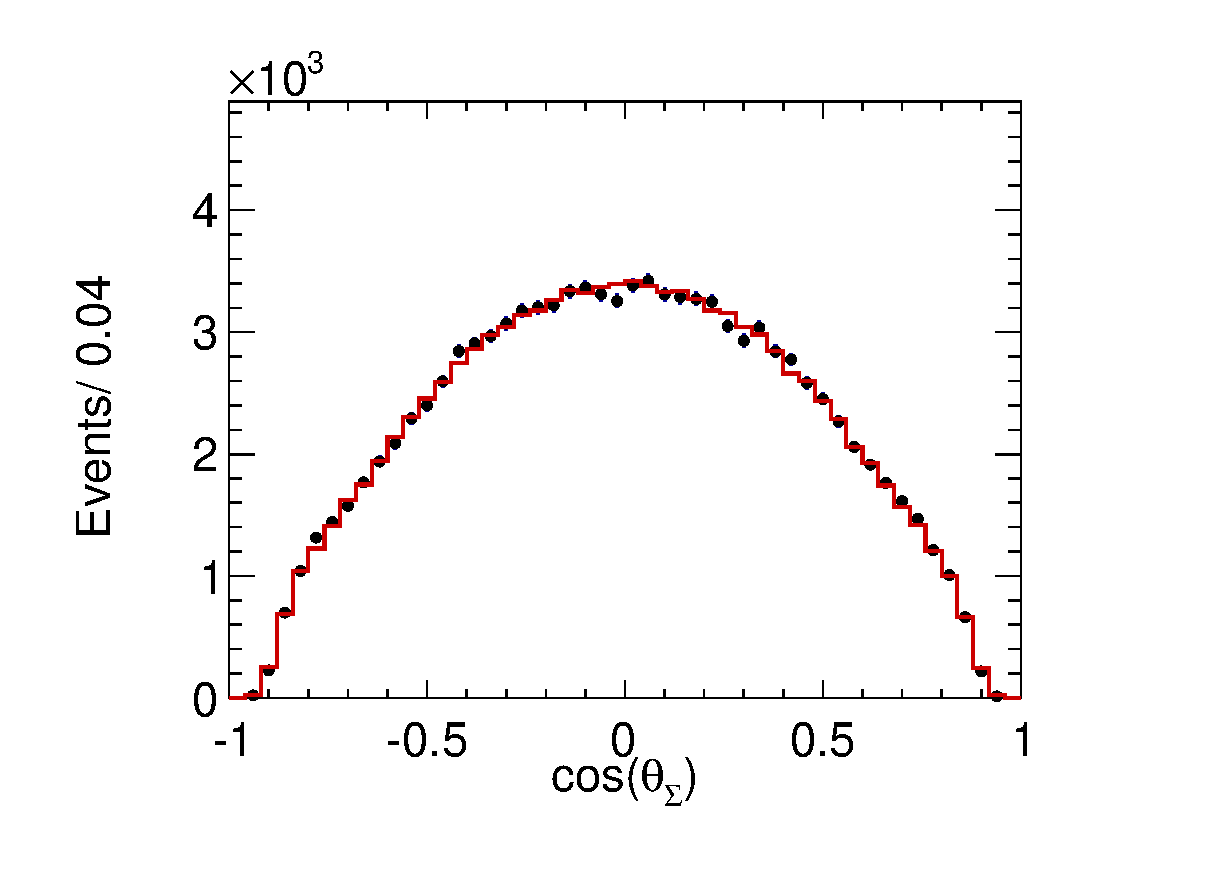
\includegraphics[width = 0.48\linewidth]{jpsi/comDataFit/t1.eps}
        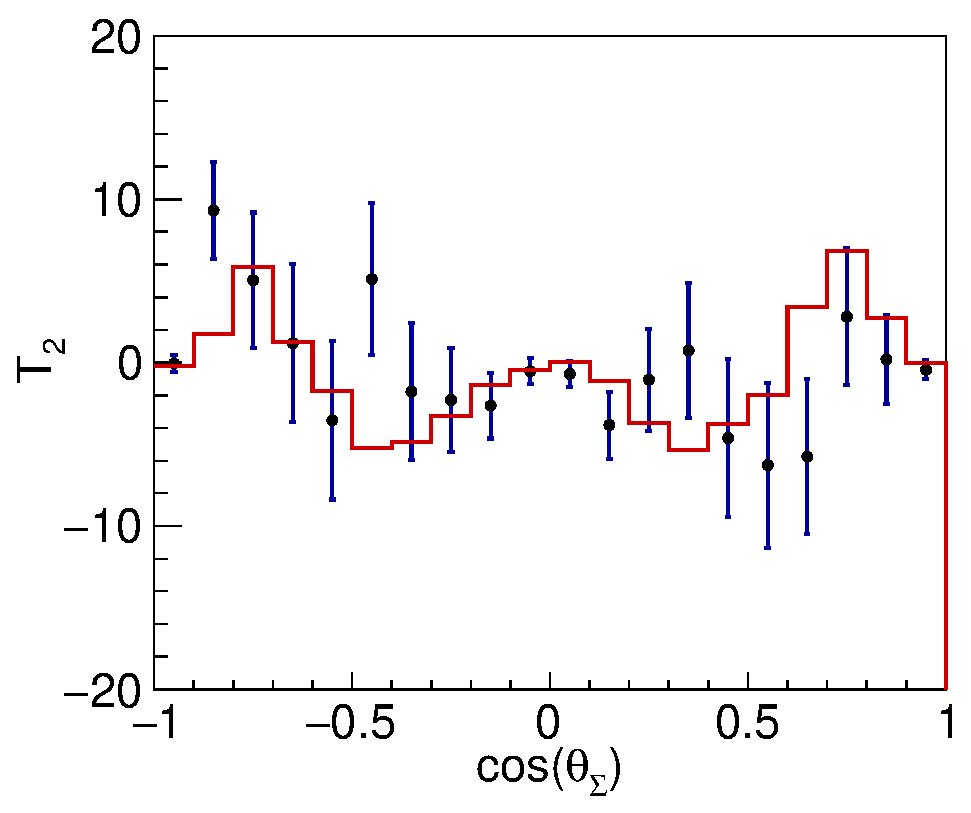
\includegraphics[width = 0.48\linewidth]{jpsi/comDataFit/t2.eps}
    }
    \mbox{%
        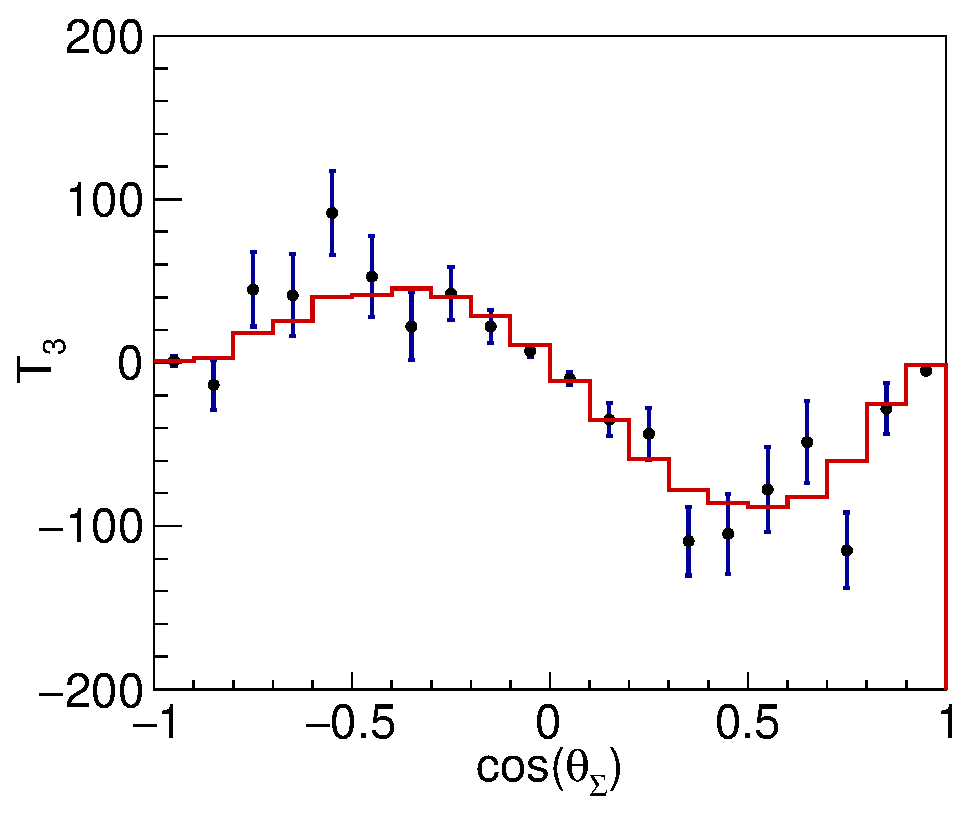
\includegraphics[width = 0.48\linewidth]{jpsi/comDataFit/t3.eps}
        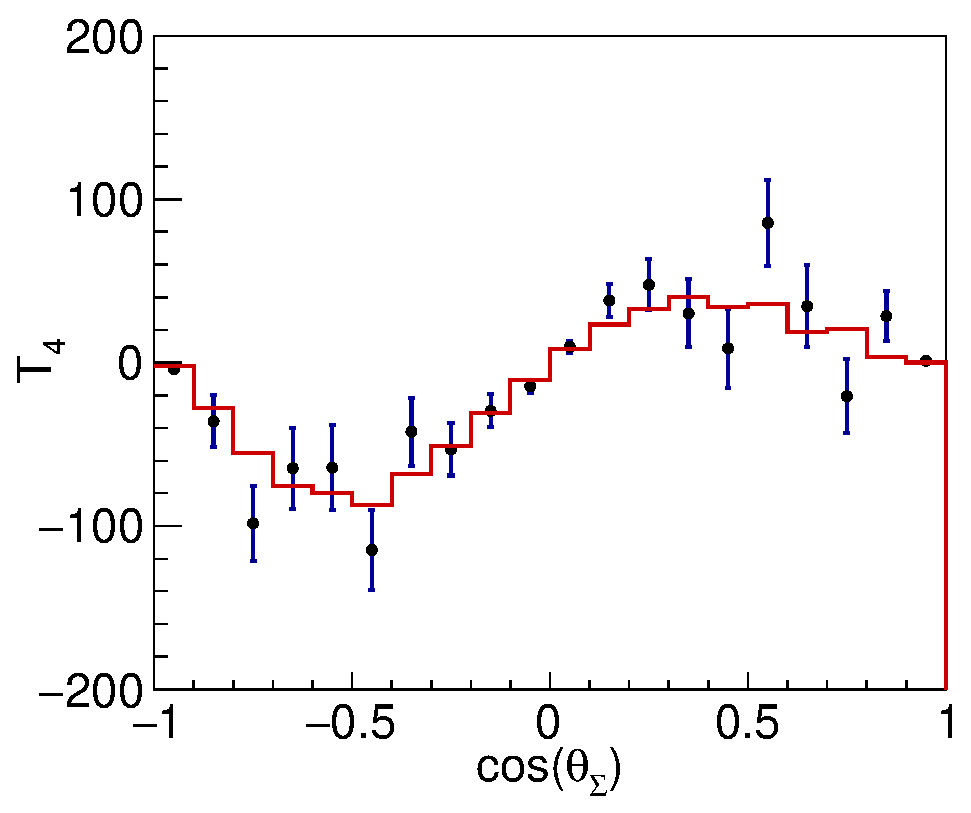
\includegraphics[width = 0.48\linewidth]{jpsi/comDataFit/t4.eps}
    }
    \mbox{%
        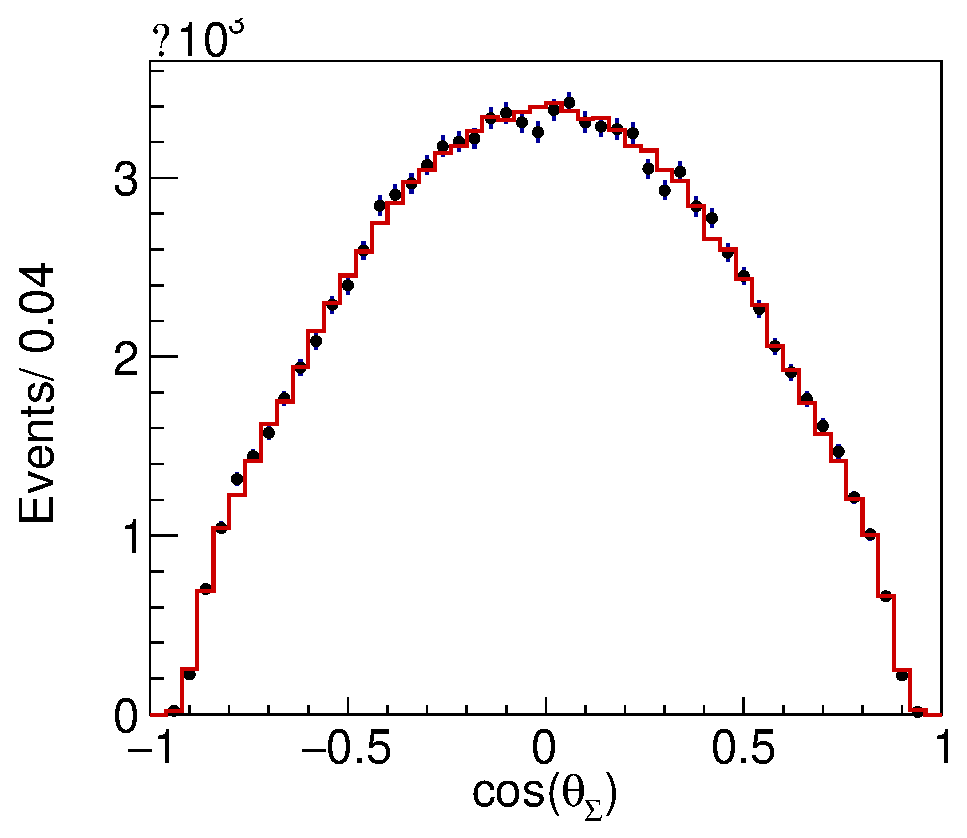
\includegraphics[width = 0.48\linewidth]{jpsi/comDataFit/CosT.eps}
    }
    \caption{数据和蒙特卡洛样本之间特征量的比较。}%
    \label{fig:compare}
\end{figure}


\begin{figure}[htbp]
    \centering
    \mbox{%
       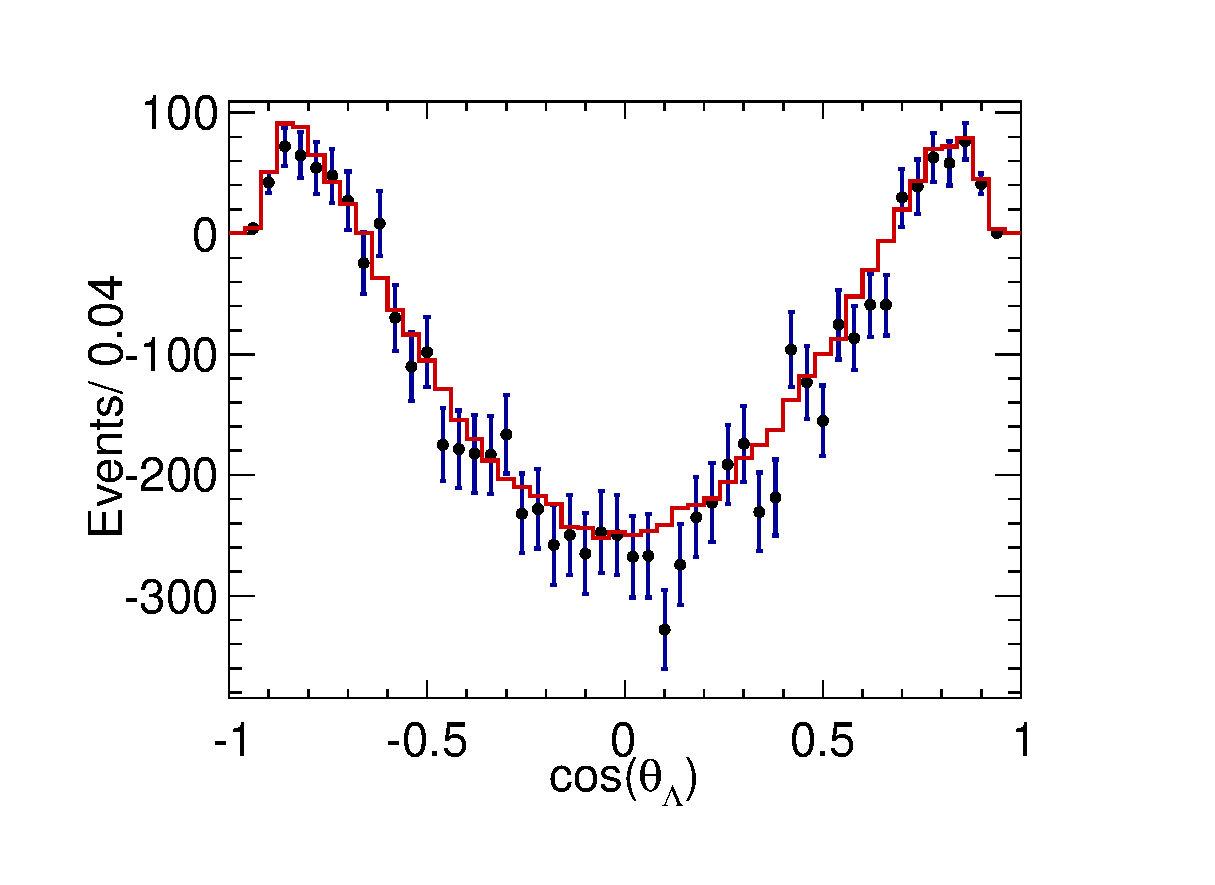
\includegraphics[width = 0.45\linewidth]{jpsi/deteParas/cosL.eps}
       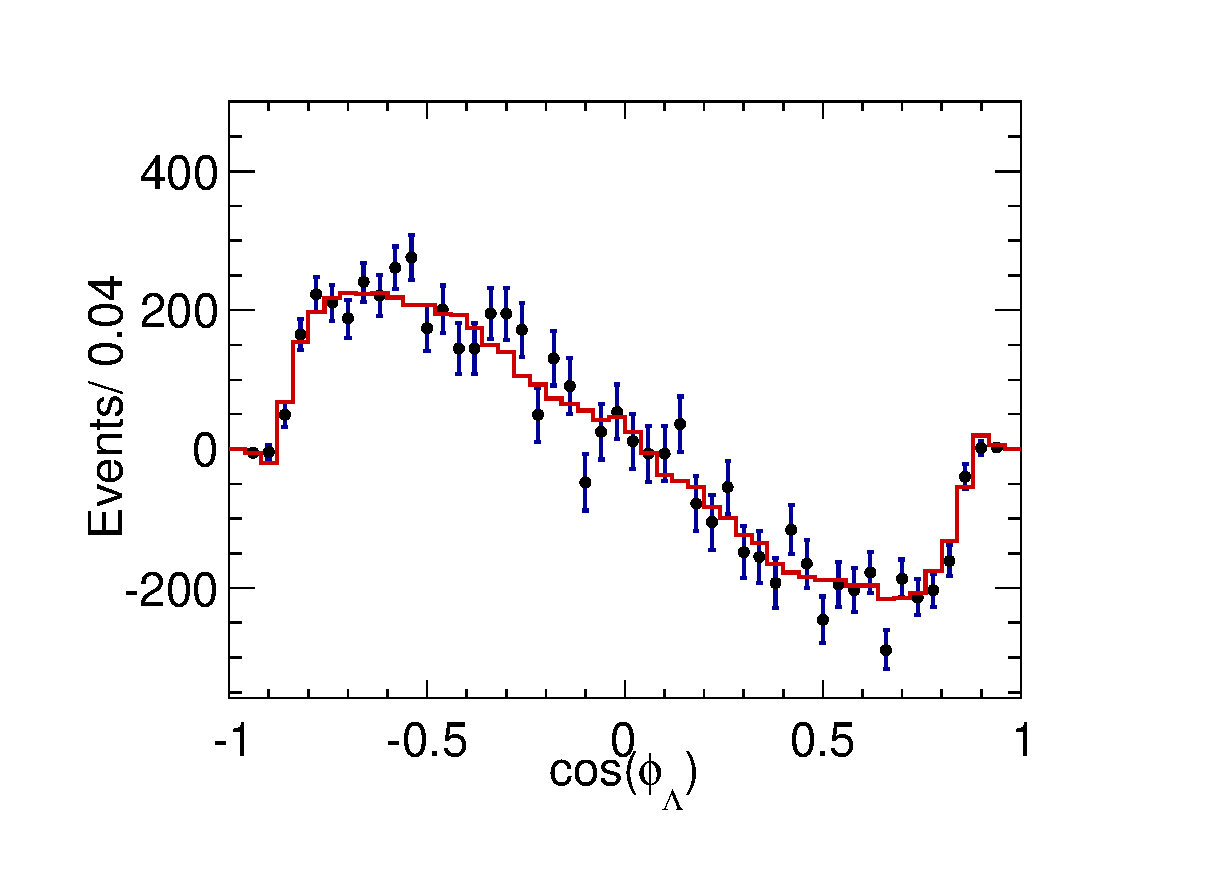
\includegraphics[width = 0.45\linewidth]{jpsi/deteParas/phiL.eps}
   }
   \mbox{%
       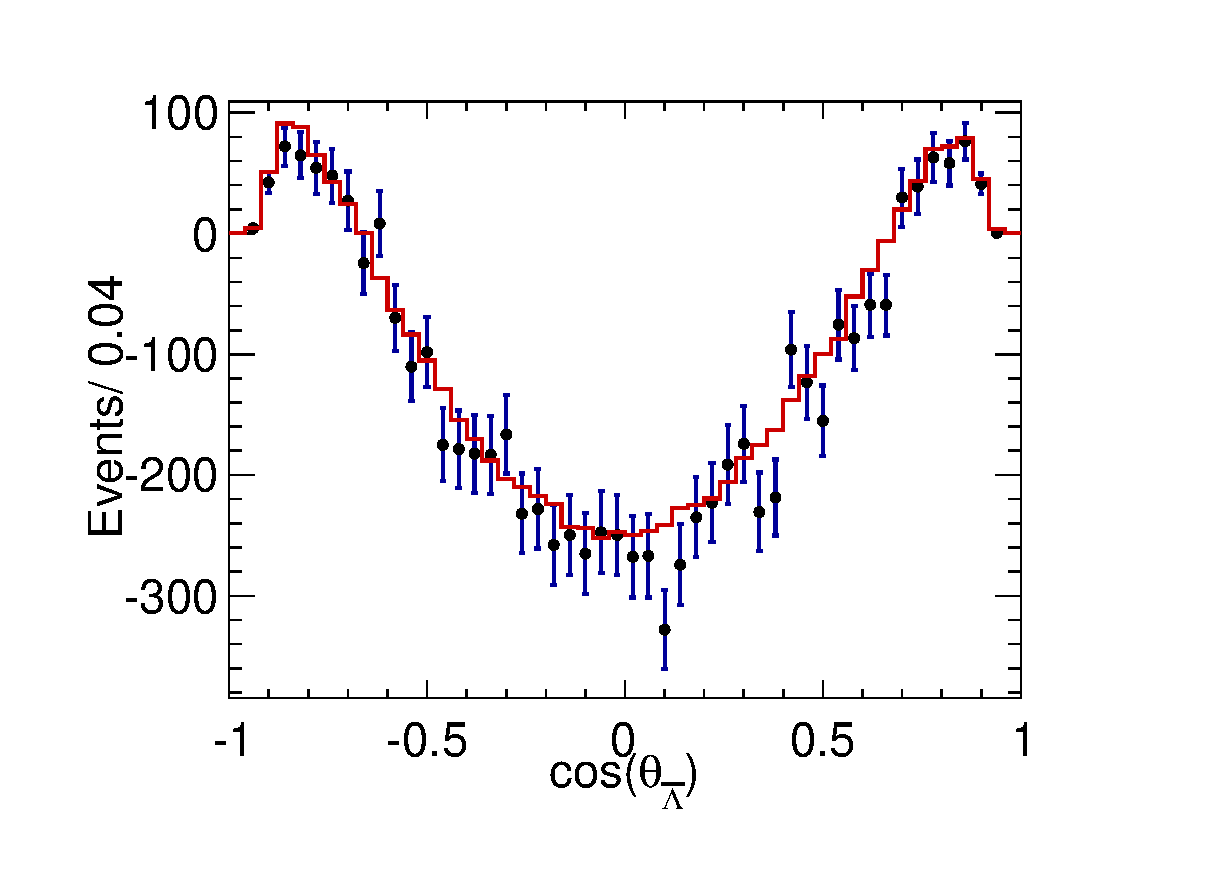
\includegraphics[width = 0.45\linewidth]{jpsi/deteParas/cosLBar.eps}
       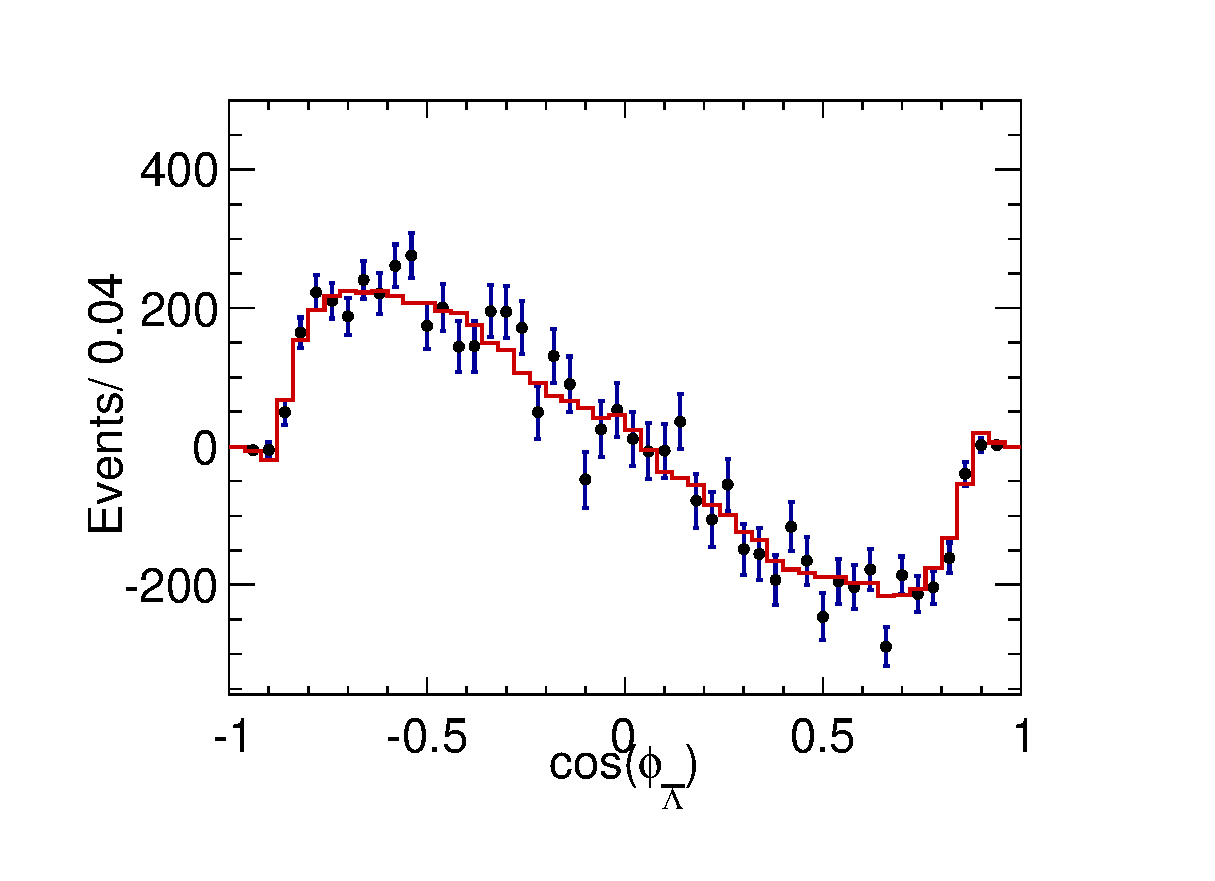
\includegraphics[width = 0.45\linewidth]{jpsi/deteParas/phiLBar.eps}
   }
   \mbox{%
       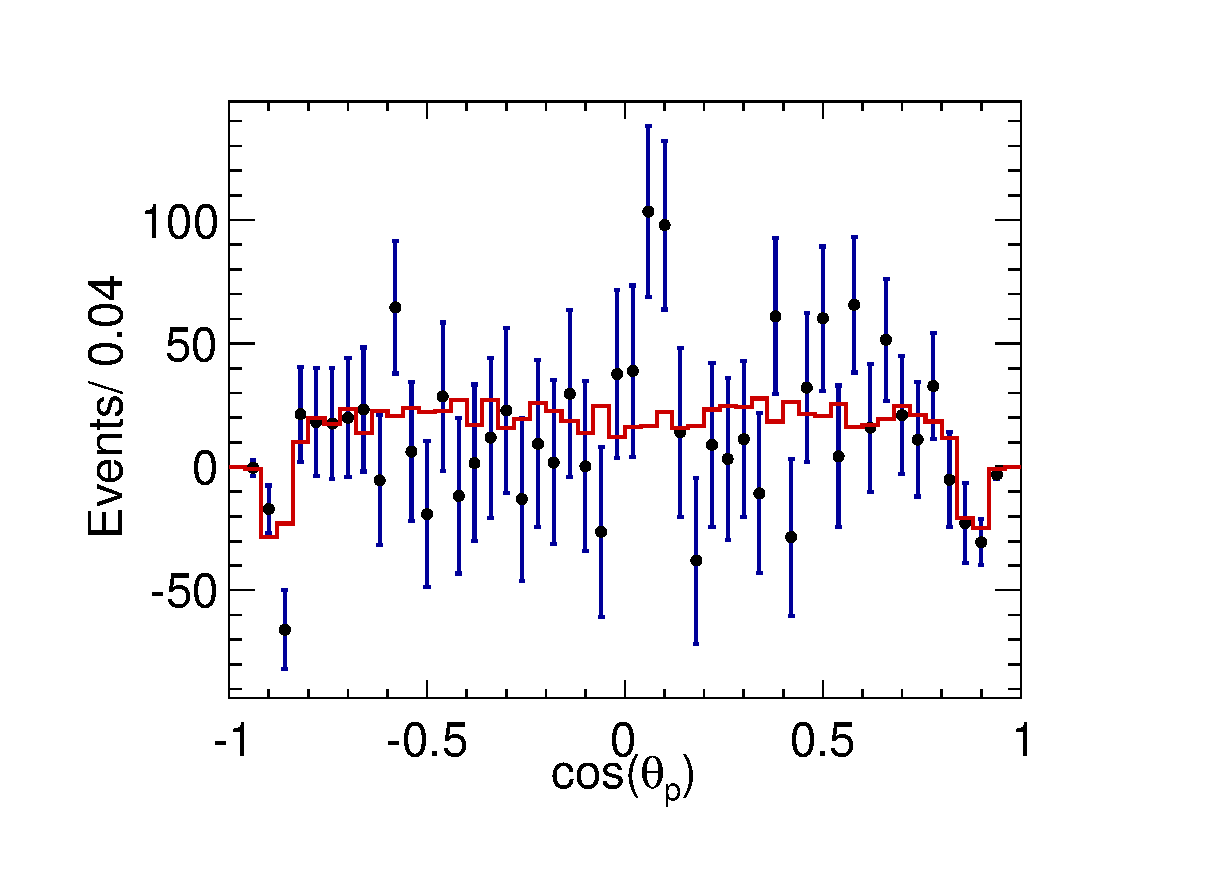
\includegraphics[width = 0.30\linewidth]{jpsi/deteParas/thetaPr.eps}
       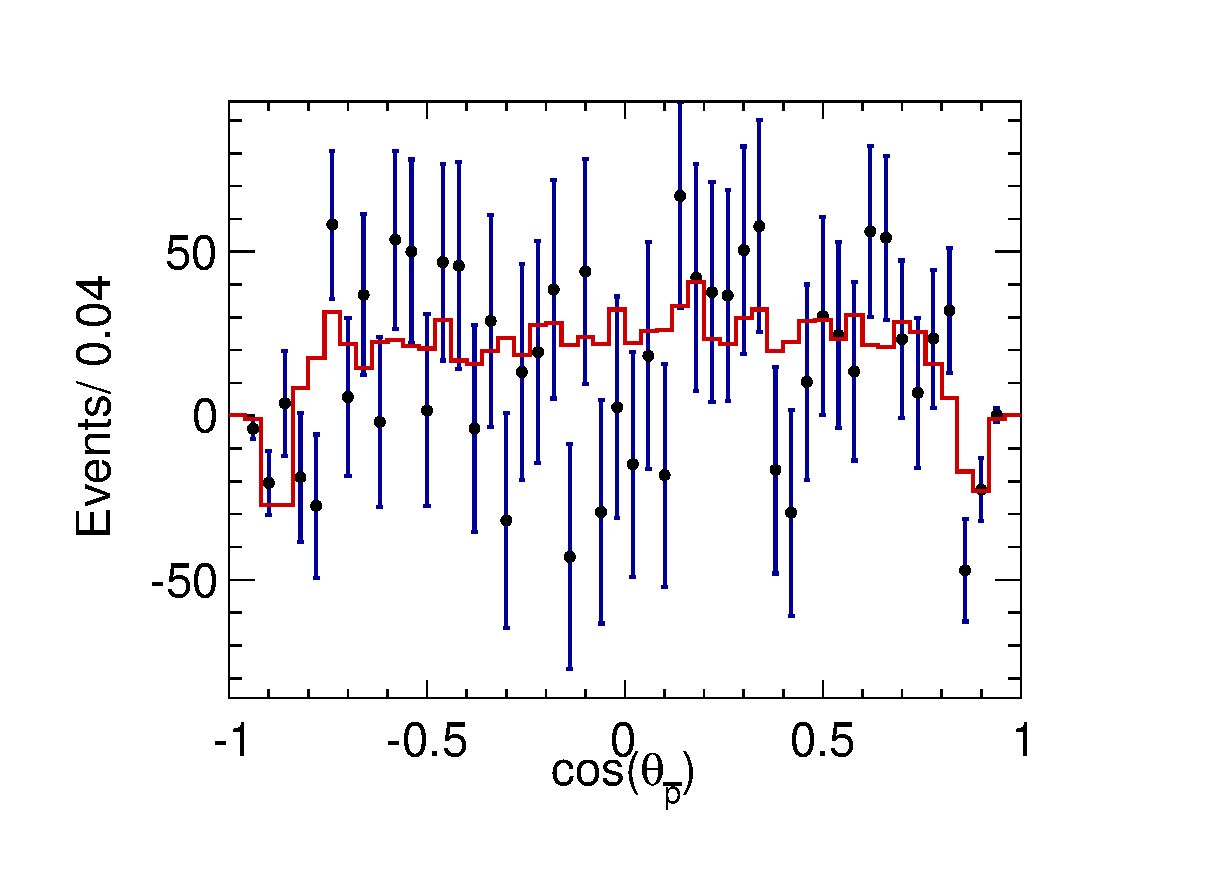
\includegraphics[width = 0.30\linewidth]{jpsi/deteParas/thetaPrBar.eps}
   }
    \caption{数据和信号蒙特卡洛样本之间的比较。}%
    \label{fig:compare2}
\end{figure}
\subsection{寻找CP破坏现象}
在小节\ref{sec:method}中,本文讨论了P宇称破坏以及CP宇称破坏与$\alpha_{\gamma}$
的关系。P宇称破坏将会导致非0的衰变参数$\alpha_{\gamma}$,因此本文要检
验$\alpha_{\gamma}$是否为0。检验的方法为将角分布公式中加入含$\alpha_{\gamma}$的
项,再重复极大似然拟合过程。

\subsubsection*{拟合结果}
按照小节\ref{sec:sigma-likelihood}的步骤,相应的$\alpha_{\gamma}$和
$\bar{\alpha}_{\gamma}$拟合值见表\ref{tab:alphaS}.

\begin{table}[htbp]
    \caption{寻找CP破坏现象的拟合结果。}%
    \label{tab:alphaS}
    \begin{center}
        \begin{tabular} {p{0.5 \linewidth} p{0.3\linewidth}}
            \toprule
            参数 & 拟合结果 \\ 
            \midrule
            $\alpha_{\gamma}$ &  $(0.7 \pm 6.6) \times 10 ^{-3}$ \\ 
            $\bar{\alpha}_{\gamma}$ & $( -7.9 \pm 6.6) \times 10^{-3}$ \\
            \bottomrule
        \end{tabular}
    \end{center}
\end{table}
\subsubsection*{CP破坏强度}
本小节首先定义观测量$O_{CP}$和$O_{C}$来衡量CP破坏和C破坏的强度,具体的定义为
\begin{equation}
    \begin{aligned}
        O_{CP}  =& \frac{\alpha_{\gamma} + \bar{\alpha}_{\gamma}}{2} \\
        O_{C}  =& \frac{\alpha_{\gamma} - \bar{\alpha}_{\gamma}}{2} 
    \end{aligned}
\end{equation}
从上式中可以得到$O_{CP} = (-3.6 \pm 4.8 \pm 0.8)\times 10^{-3}$,
$O_{C} = (0.43 \pm 4.6 \pm 0.8)\times 10^{-3}$,其中的第一项误差为统计误差,
第二项误差为系统误差,后续的章节中将详细讨论系统误差的来源。从中可以看出CP破坏
强度在1$\sigma$内和0一致,并为观测到显著的CP破坏现象,类似了也没有显著的C破坏
现象。

%\subsection{系统误差研究}
\section{系统误差研究}%
\label{sec:sigma0-sys-unc}
系统误差按来源可以分为如下的五种:

\begin{itemize}
    \item 末态带电粒子的寻迹;
    \item 光子的重建;
    \item $\Lambda$和$\bar{\Lambda}$的次级顶点拟合;
    \item 运动学拟合;
    \item 本底估计。
\end{itemize}
每种主要的系统误差来源都可以归为两类,其一通过影响效率函数进而对拟合结果产生
影响,其二则不会影响效率函数本身,但是影响似然函数$S$,比如本底的估计。
第一类系统误差只会影响小节\ref{sec:sigma0-likelihood}中归一化因子$N$的估计,
在计算归一化因子的时候本文选择给予每个蒙特卡洛事例一定的权重以补偿数据和蒙特卡洛样本之间的
效率差异,从而将间接的修正效率函数,具体计算的公式为
\begin{equation}
    \label{eq:vary-weight-sigma0}
    N' = \frac{1}{n}  \sum_{i}^{MC} weight_{i} \cdot 
    \mathcal{P}(\vec{\theta_{i}}; \vec{\alpha}),
\end{equation}
式中$weight_{i}$代表第$i$个蒙特卡洛样本的权重,应如此计算
\begin{equation}
    weight  \equiv \frac{\epsilon_{\rm data}}{\epsilon_{\rm MC}} ,
\end{equation}
其中的$\epsilon_{\rm data}$和$\epsilon_{\rm
MC}$分别是数据和蒙特卡洛中的效率函数。这些效率一般从控制样本中得到,
比如质子的寻迹效率。
第二类系统误差不会改变效率曲线的形状,但也会影响拟合的结果,比如本底的估计。
一般通过估计策略的变动拟合结果也随之改变,因此本文采用变化策略,把拟合结果的变动
作为系统误差。在下节将讨论具体的方法。
\subsection{带电粒子的寻迹}%
\label{sec:Tracking-unc-sigma0}
末态的带电粒子种类包括质子和$\pi$介子。一般需要通过控制样本来研究带电粒子的寻迹
效率。控制样本选取的原则包括:大样本、低本底。研究质子寻迹效率的一个理想样本
是:
$J/psi \to p \bar{p} \pi^{+} \pi^{-}$。研究的精神是:
\begin{itemize}
    \item 用三个带电末态$\bar{p} \pi^{+} \pi^{-}$标记质子,这样得到的被标记质子
        就是所谓的控制样本。由于带电粒子的动量分辨好,本底低,因此被标记质子的
        运动学信息能够被精确的得到。另一方面,很容易通过拟合丢失不变质量谱
        确定质子的数目。
    \item 根据被标记质子的运动学信息去寻找一条与之相符的带电径迹。一般常常利用
        飞行方向的信息,两者夹角小于20度认为寻迹正确。
\end{itemize}
宋娇娇博士对质子和$\pi$介子的寻迹效率进行了研究\cite{PID:jiaojiao},
在她研究得到的效率的基础上,本文对式\ref{eq:vary-weight-sigma0}中的权重进行相应
的变动。本文把相空间积分蒙特卡洛样本按质子和$\pi$介子的动量和极角划分成
若干区间,其中动量区间的宽度为100 MeV$/c$,极角 ($\cos\theta$)的区间宽度为0.2。
本文假设任意一个区间内的权重因子服从高斯分布,$\sigma$按误差传递公式确定。
为了确定修正带来的误差,本文选择做多次实验,每次实验的中的每个区间内的权重因子
均按高斯分布进行随机抽取,最终得到一系列拟合结果。经过400次实验后,得到的拟合
结果见图\ref{fig:fit-value-track}。如图所示,拟合结果的中心值应服从正态分布,
为了验证这一点,本文用高斯函数对这400次实验做了拟合,蓝色的实线是拟合的结果。
本文选择把高斯函数的中心值作为经过径迹效率修正后的报告值,高斯函数的$\sigma$
作为径迹效率修正的系统误差,这项误差总结在表\ref{tab:unc-track-sigma0}中。

% /besfs/groups/jpsi/jpsigroup/user/maxx/Jpsi/SS/664/noDangCut/Uncertainty/trackingAndPid/
\begin{figure}[htbp]
    \centering
    \mbox{%
        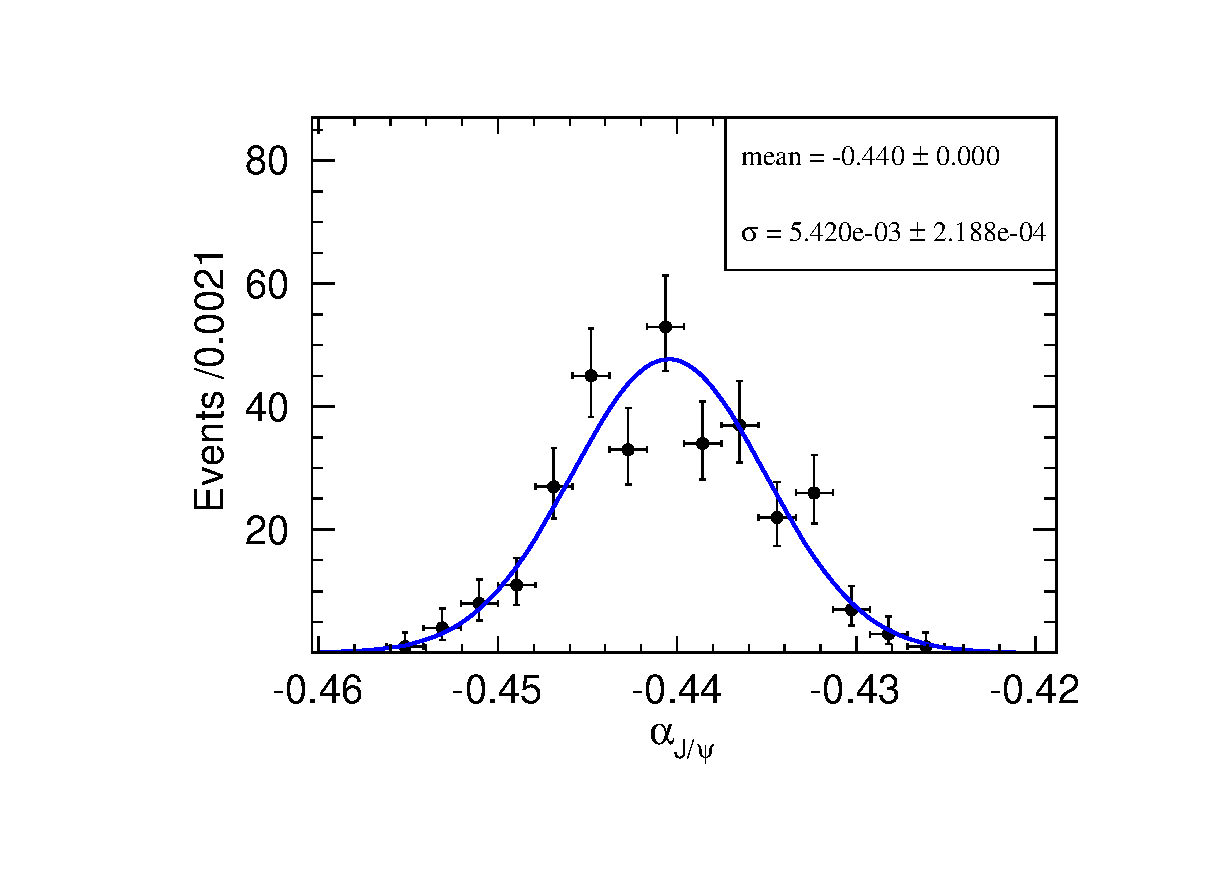
\includegraphics[width = 0.48\linewidth]{jpsi/unc/trkalpha.eps}
        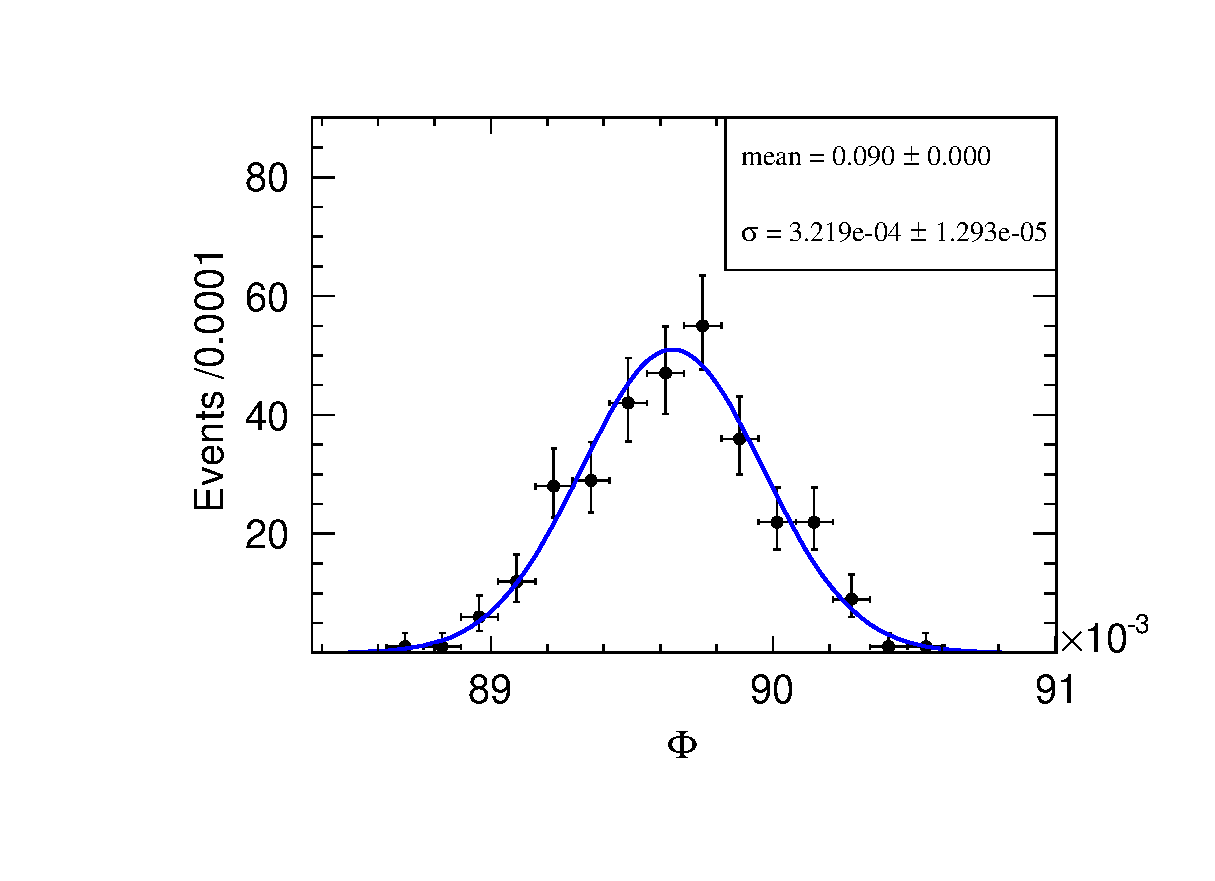
\includegraphics[width = 0.48\linewidth]{jpsi/unc/trkphi.eps}
    }
    \mbox{%
        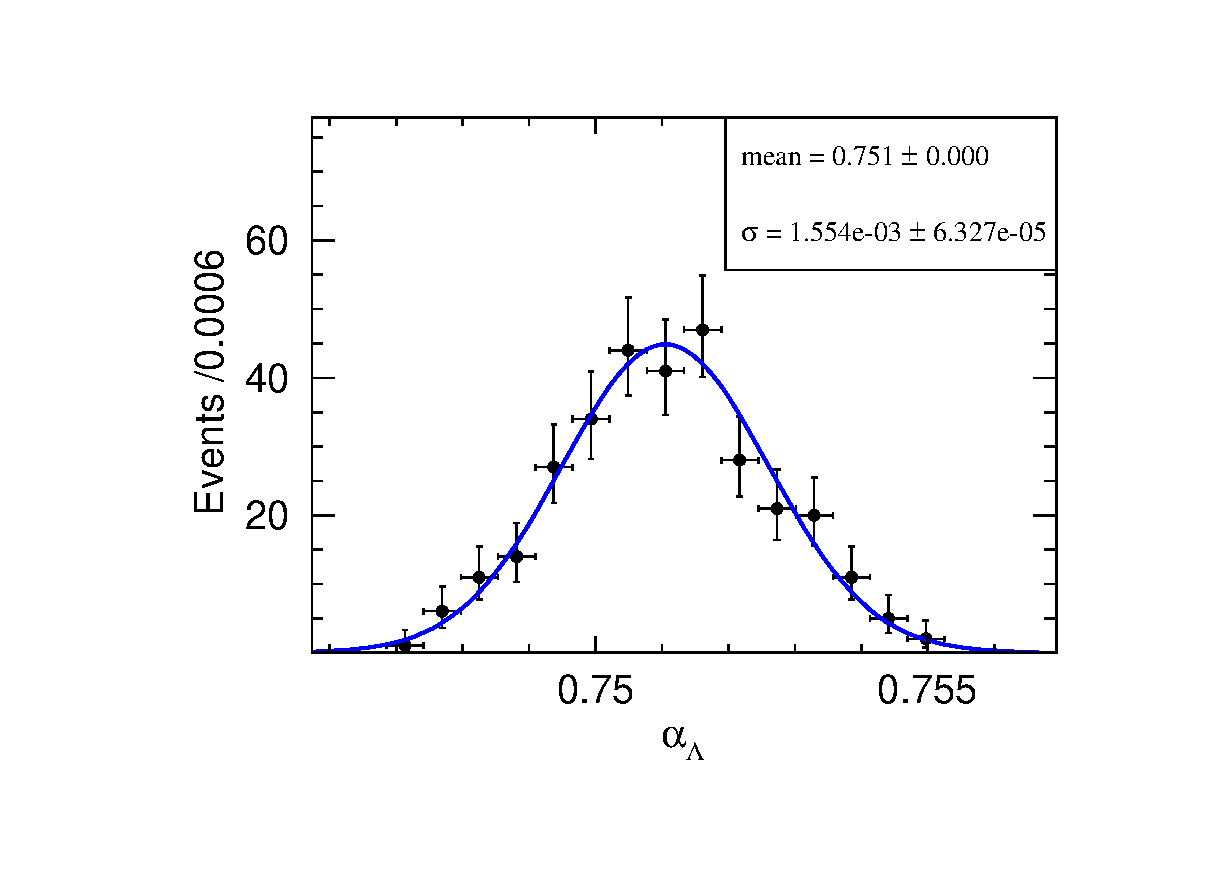
\includegraphics[width = 0.48\linewidth]{jpsi/unc/trkalphaL.eps}
        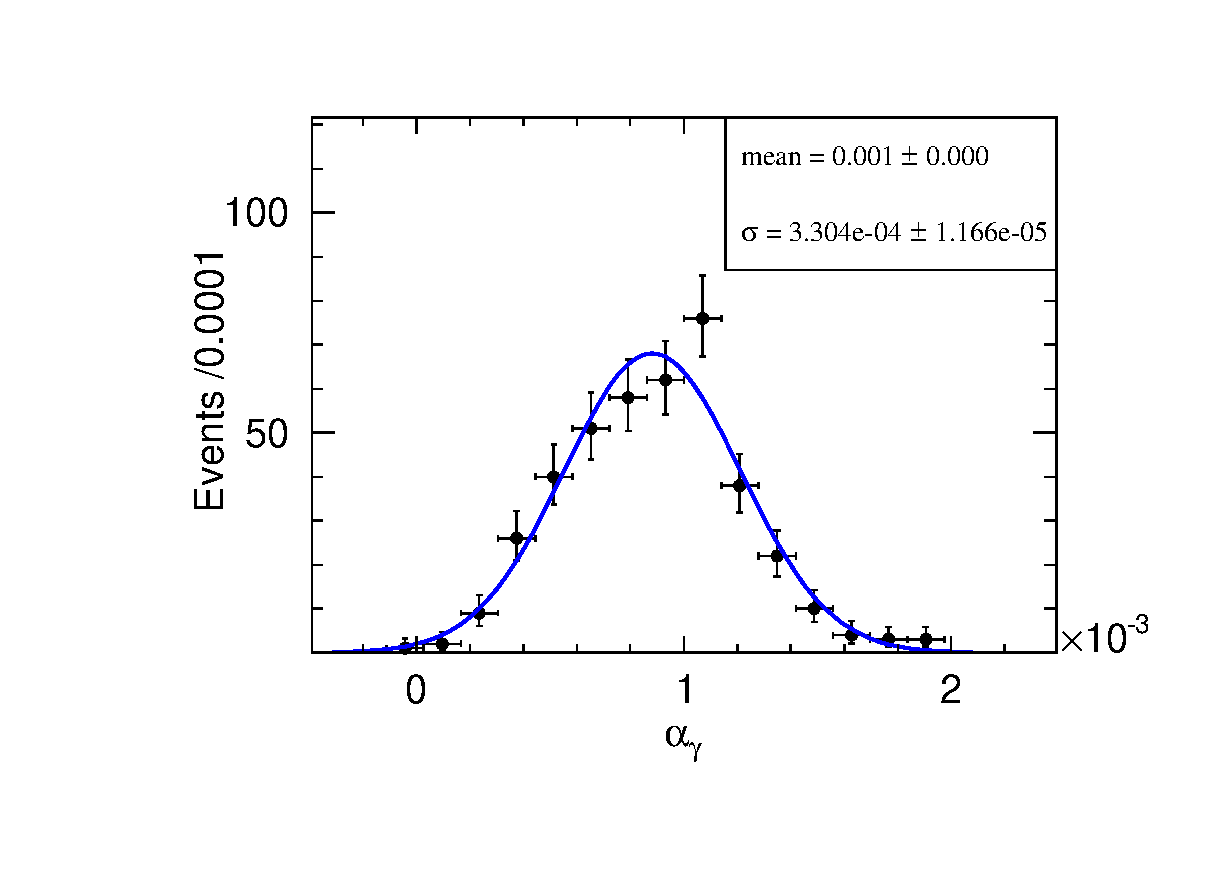
\includegraphics[width = 0.48\linewidth]{jpsi/unc/trkalphagamma.eps}
    }
    \mbox{%
        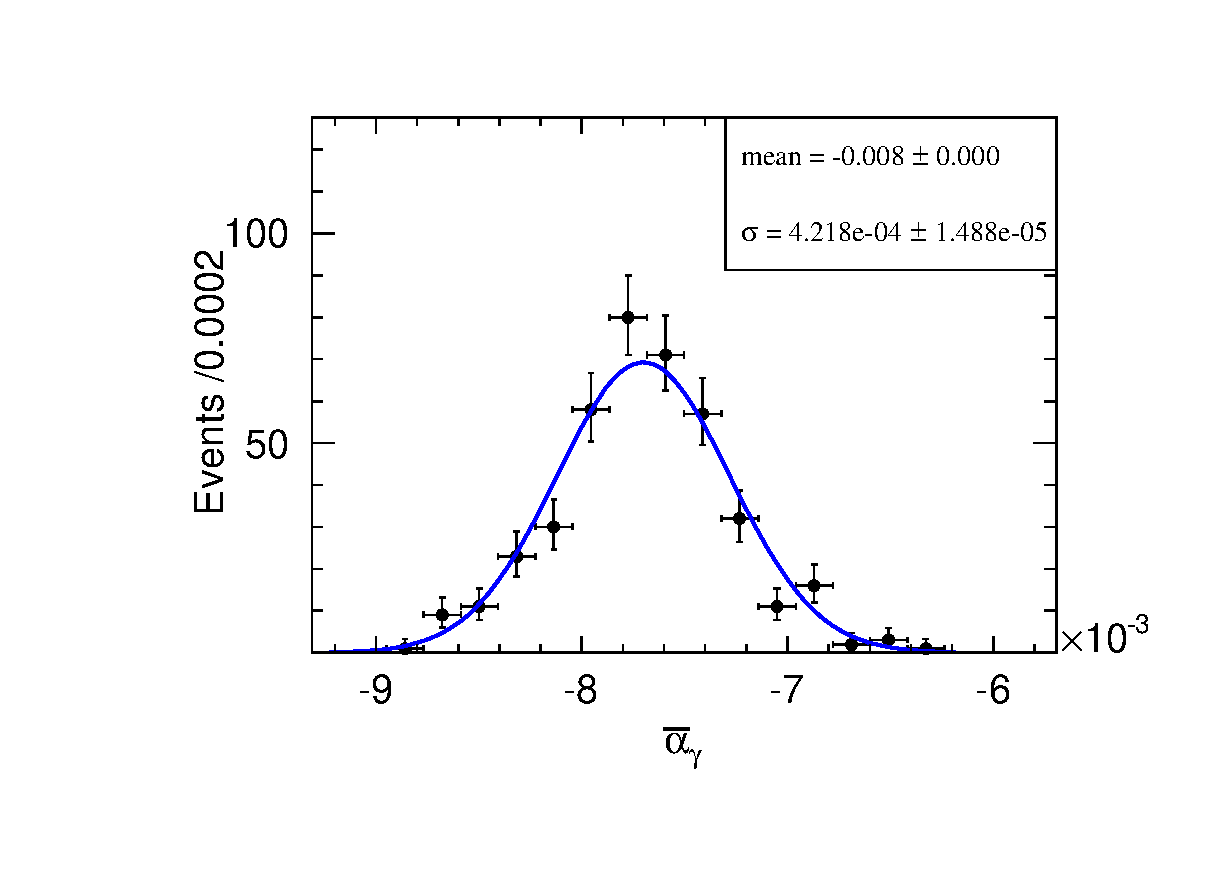
\includegraphics[width = 0.48\linewidth]{jpsi/unc/trkalphagammaBar.eps}
    }
    \caption{%
        随机变动参数$weight$得到的多次实验结果。本文对图中400次拟合结果做了拟合。
        蓝色的实线表示拟合的结果,相关的参数结果标注在图的右上角。
    }%
    \label{fig:fit-value-track}
\end{figure}


\begin{table}[htbp]
    \caption{寻迹效率修正的系统误差。}%
    \label{tab:unc-track-sigma0}
    \begin{center}
        \begin{tabular} {p{0.5 \linewidth} p{0.3 \linewidth}}
            \toprule 
            参数 & 系统误差 (\%) \\
            \midrule
            $\alpha_{J/\psi}$  & 1.3 \\
            $\Phi$             & 0.36 \\
            $\alpha_{\Lambda}$ & 0.21 \\
            \bottomrule
        \end{tabular}
    \end{center}
\end{table}

\subsection{光子重建}%
\label{sec:photon-rec-Sigma0}
光子重建效率与极角和能量有关,Vindy博士对光子重建的效率进行了系统的研究,在他
的工作的基础,本文按光子的极角和能量对效率曲线进行了修正,并得到了相应的系统
误差。在Vindy博士研究成果的基础上,本节对式\ref{eq:vary-weight-sigma0}中
的$weight$进行相应的随机变动。做了400变动后,得到的拟合参数的分布
如图\ref{fig:fit-value-photon}所示,采取和小节\ref{sec:Tracking-unc-sigma0}
相同的策略得到的系统误差总结在表\ref{tab:unc-photon-Sigma}中。
% /besfs/groups/jpsi/jpsigroup/user/maxx/Jpsi/SS/664/noDangCut/Uncertainty/gammaRec/
\begin{figure}[htbp]
    \centering
    \mbox{%
        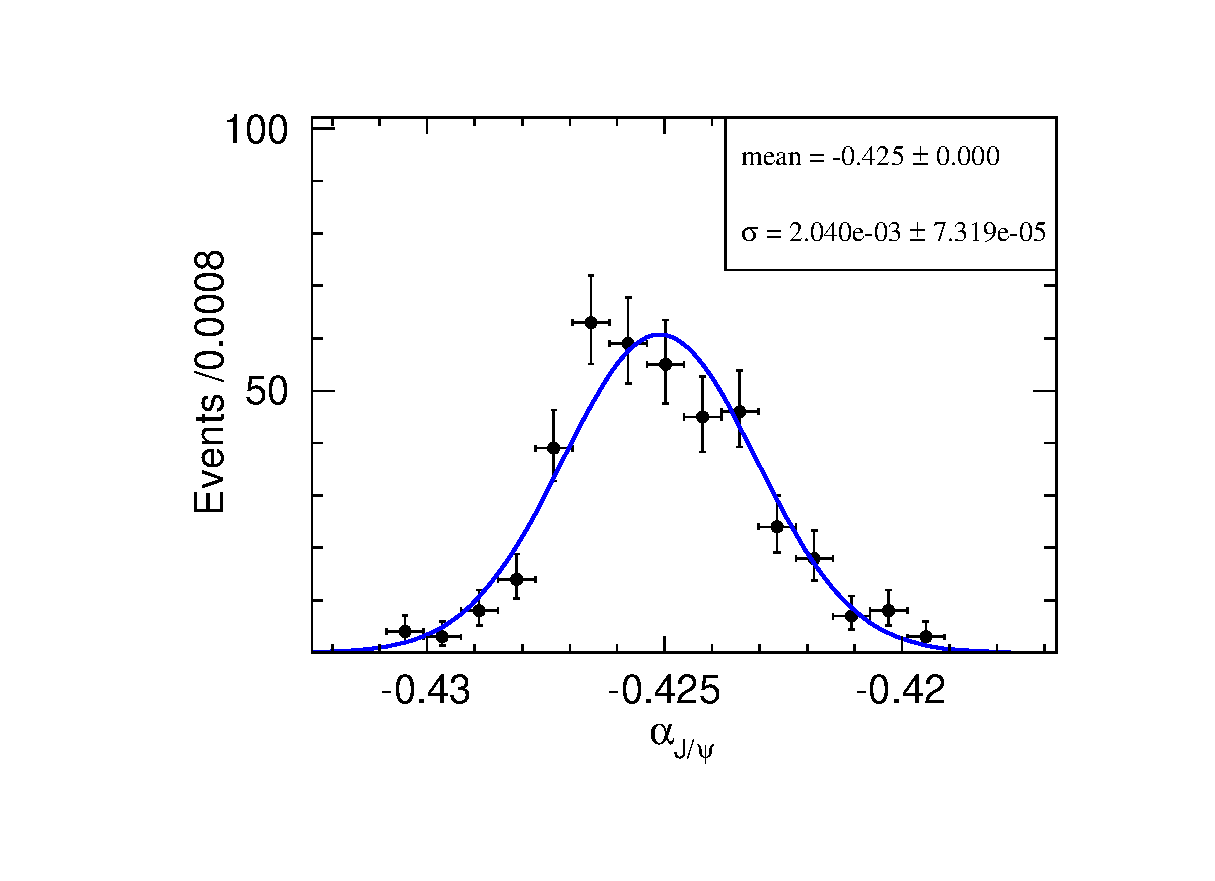
\includegraphics[width = 0.48\linewidth]{jpsi/unc/photonalpha.eps}
        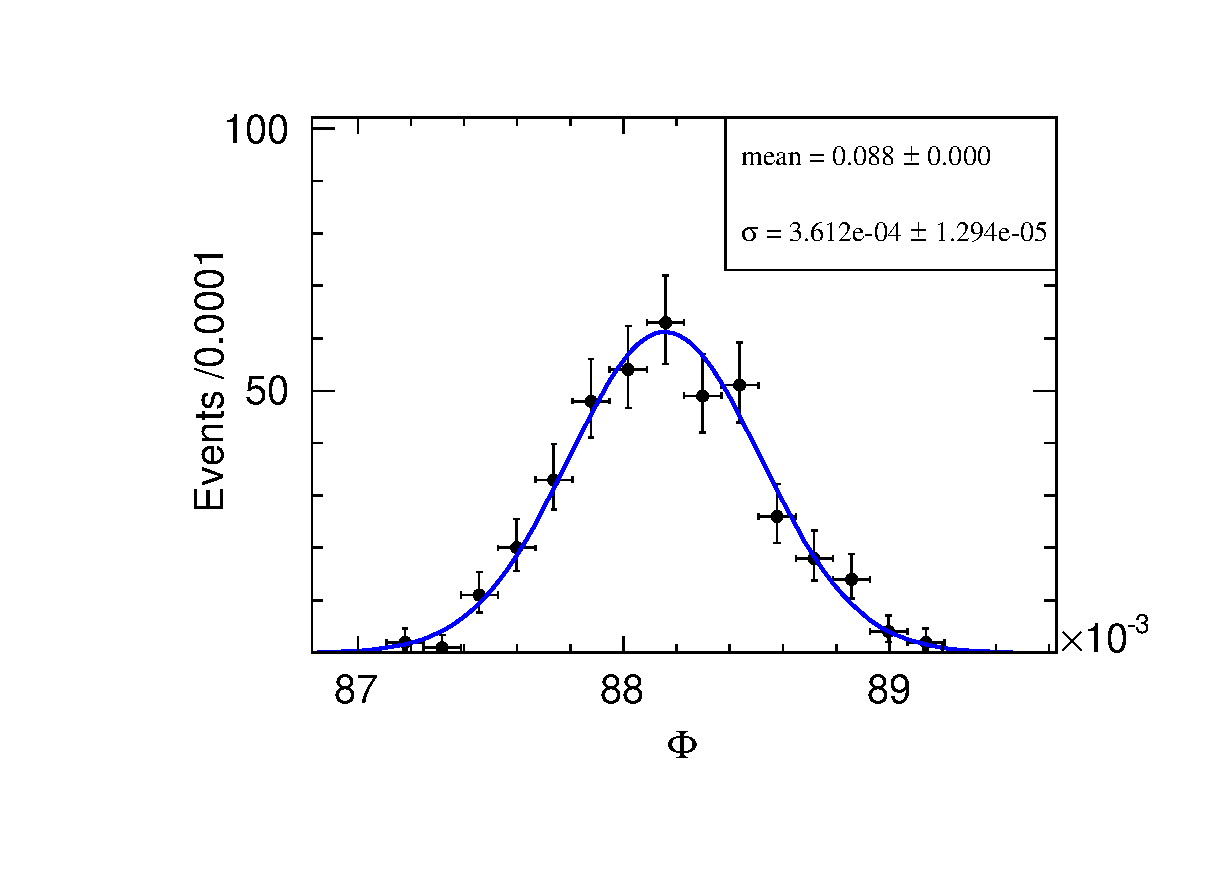
\includegraphics[width = 0.48\linewidth]{jpsi/unc/photonphi.eps}
    }
    \mbox{%
        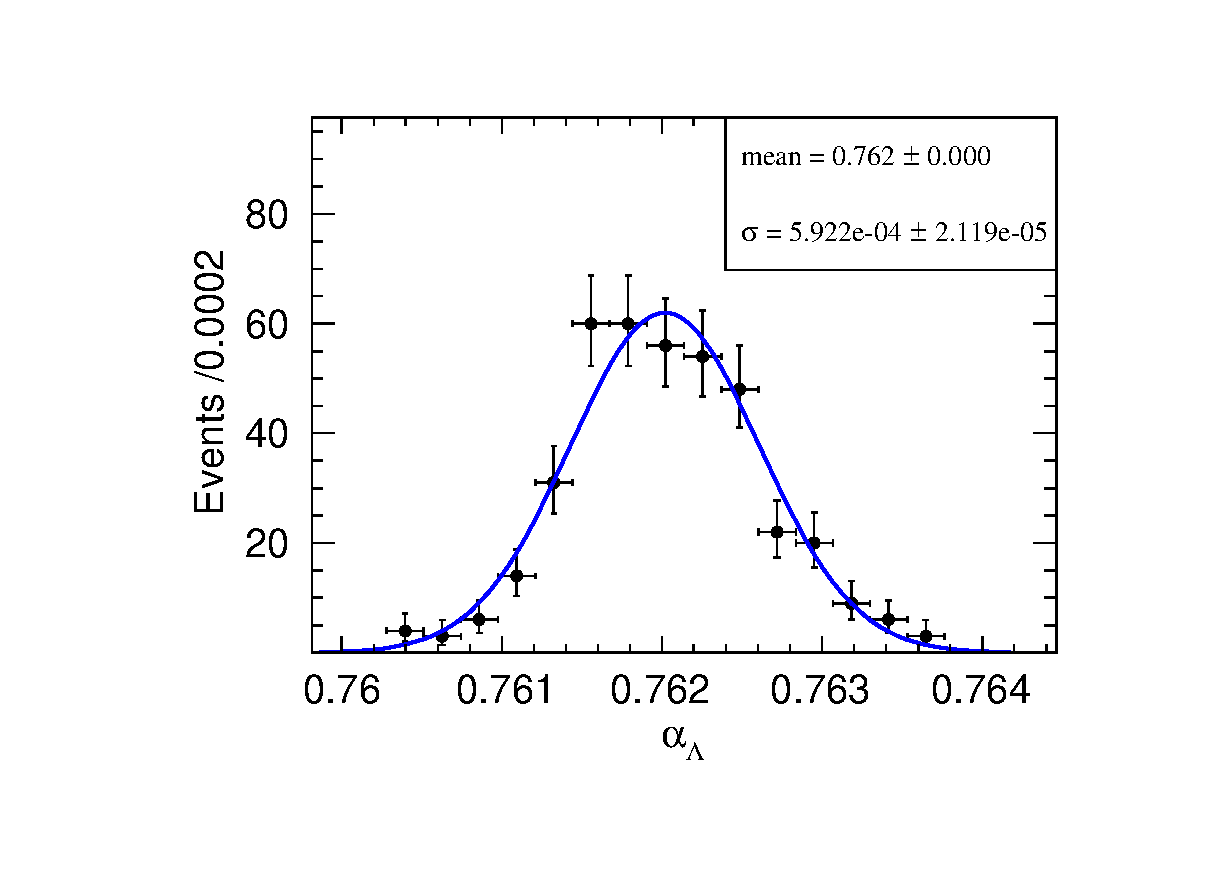
\includegraphics[width = 0.48\linewidth]{jpsi/unc/photonalphaL.eps}
        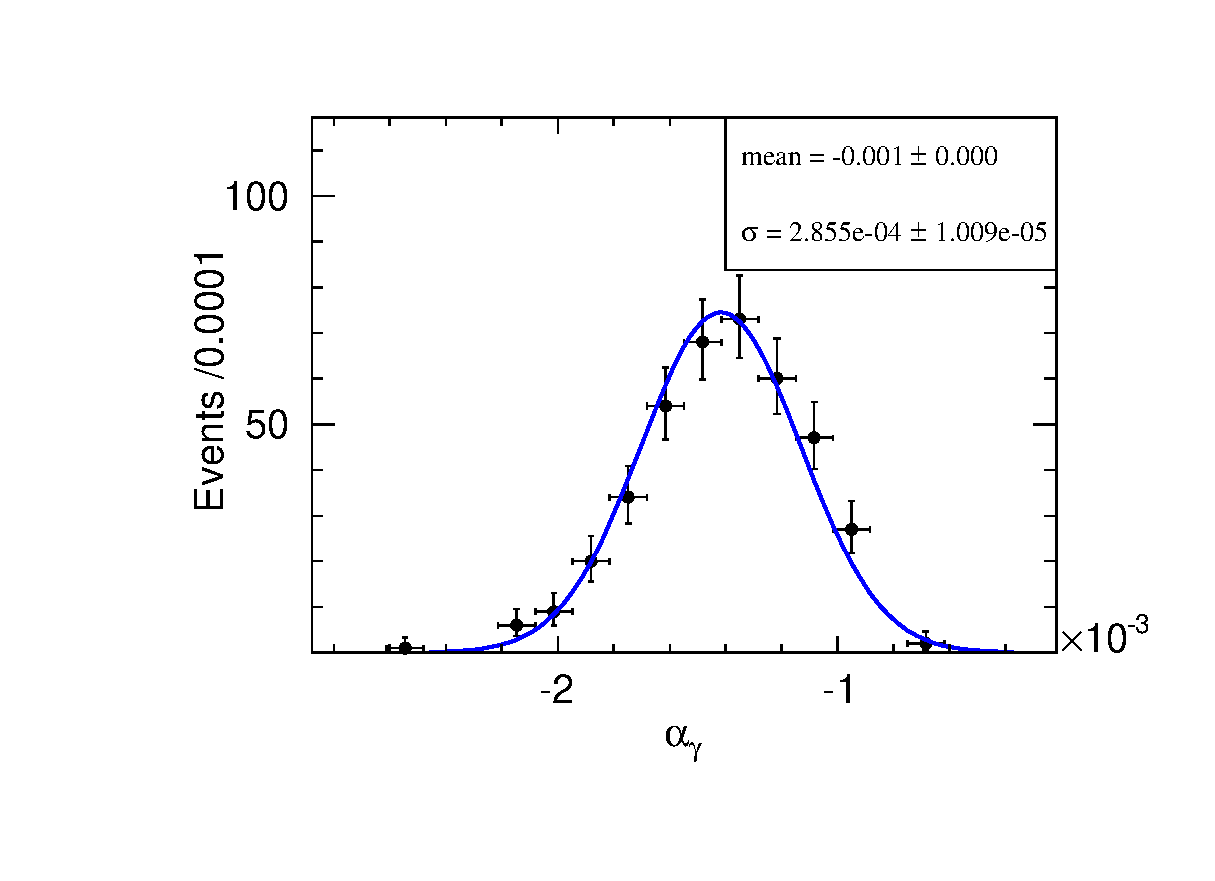
\includegraphics[width = 0.48\linewidth]{jpsi/unc/photonalphagamma.eps}
    }
    \mbox{%
        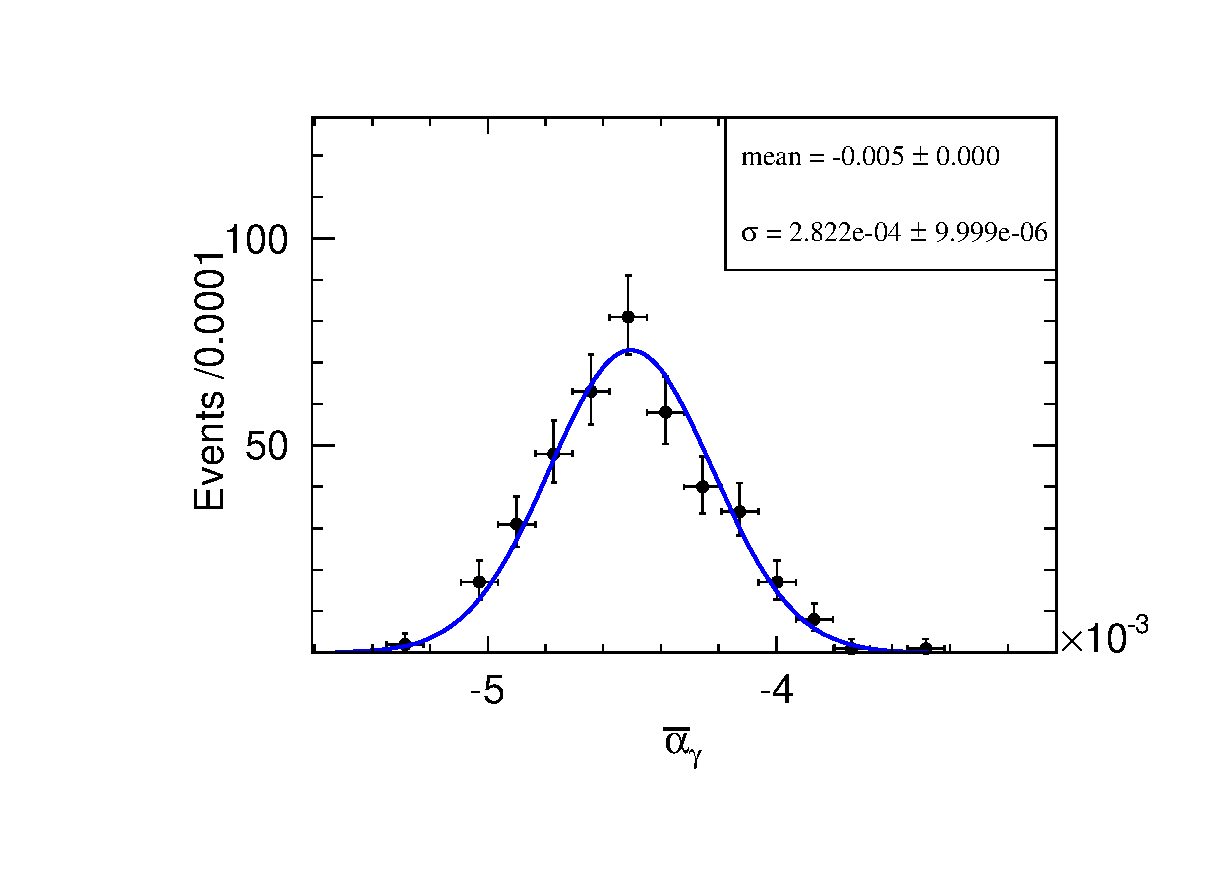
\includegraphics[width = 0.48\linewidth]{jpsi/unc/photonalphagammaBar.eps}
    }
    \caption{%
        对光子重建效率进行400次加权测试得到的拟合参数分布。带误差棒的黑色的
        带误差棒的点表示拟合的结果,蓝色的实线为用高斯函数拟合的结果。
    }%
    \label{fig:fit-value-photon}
\end{figure}

\begin{table}[htbp]
    \caption{光子重建带来的系统误差总结。}%
    \label{tab:unc-photon-Sigma}
    \centering
    \begin{tabular} {p{0.5 \linewidth} p{0.4 \linewidth}}
        \toprule 
        衰变参数 & 系统误差 (\%) \\
        \midrule
        $\alpha_{J/\psi}$  & 0.48 \\
        $\Phi$             & 0.41 \\
        $\alpha_{\Lambda}$ & 0.78 \\
        \bottomrule
    \end{tabular}
\end{table}

\subsection{$\Lambda$的次级顶点重建}
为了研究$\Lambda$的次级顶点重建的效率,本节挑选了控制样本$J/\psi 
\to pK^{-} \bar{\Lambda}$及$J/\psi \to \Lambda \bar{\Lambda}$来确定数据和
蒙特卡洛样本中的重建效率。加上详细的叙述。

\subsection{运动学拟合}
本节选择控制样本$J/\psi \to p \bar{p} \pi^{+}\pi^{-}\pi^{0}$来确定运动学拟合
的效率曲线,这个控制样本的特点是末态和信号高度相同,能够有效的揭示出数据
和蒙特卡洛之间的差异。加上描述。

\subsection{本底的影响}
为了确定本底带来的影响,本节采取去掉公式\ref{eq:final-likehood}中的本底项
重新进行拟合并把和保留本底项的结果进行比较,两者之间的差异作为系统误差。

%\subsection{系统误差小节}
至此所有的系统误差都得到了精细的研究,每项的系统误差和总的系统误差见
表\ref{tab:unc-summary}.

\begin{table}[htbp]
    \caption{系统误差的总结表。}%
    \label{tab:unc-summary}
    \centering
    \begin{tabular} {p{0.3 \linewidth} p{0.1\linewidth} p{0.1\linewidth} 
        p{0.1\linewidth} p{0.1\linewidth} p{0.1\linewidth} }
        \toprule
        \multirow{2}{*} {来源}
        & \multicolumn{5}{c}{误差 (\%)} \\ 
        \cline{2-6}
        & $\alpha_{J/\psi}$ & $\Phi$ & $\alpha_{\Lambda}$ 
        & $\alpha_{\gamma}*$ & $\bar{\alpha}_{\gamma}*$ \\
        \midrule
        寻迹 & $1.3$ & $0.36$ & $0.21$  & $0.3 \times 10^{-4}$ 
        & $4.2 \times 10^{-4}$ \\
        光子重建 & $0.48$ & $0.41$ & $0.78$
        & $2.8 \times 10^{-4}$ & $2.8 \times 10^{-4}$\\
        $\Lambda$的次级顶点重建 & $2.8$ & $0.53$ & $0.37$ 
        & $4.2 \times 10^{-4}$ & $4.2 \times 10^{-4}$ \\
        运动学拟合 & $2.0$ & $0.57$ & $0.41$
        & $6.0 \times 10^{-4}$ & $5.9\times 10^{-4}$ \\
        本底估计 & $0.80$ & $0.58$ & $0.07$
        & $7.6 \times 10^{-4}$ & $7.9 \times 10^{-4}$ \\
        \midrule
        总和 & $3.8$ & $1.1$ & $1.0$  & $1.2 \times 10^{-3}$ & 
        $1.2 \times 10^{-3}$ \\
        \bottomrule
    \end{tabular}
\end{table}
